\chapter{Cherenkov angle resolution by mirror-pair}
In this chapter the Cherenkov angle resolution per mirror-pair is studied.\\
The 2D histograms of the Cherenkov angle resolution $\Delta \theta$ vs. azimuthal angle $\Phi$ for fully aligned mirrors are projected onto the Cherenkov angle resolution. Then a function consisting of a Gaussian representing the signal contribution and a polynomial of order 2 representing the background contribution is fitted to the Cherenkov angle resolution distribution: 
\begin{equation}
f(x) = a \cdot e^{-0.5 \cdot \left( \frac{x - \mu}{\sigma}\right)^2} + b + c \cdot x + d \cdot x^2
\label{eq:1}
\end{equation}
($a$, $b$, $c$, $d$, $\mu$ and $\sigma$ are determined by the fit).\\
The width of the fitted Gaussian represents the Cherenkov angle resolution.\\
\begin{figure}[!h]
	\vspace*{-0.cm}
	\begin{center}
		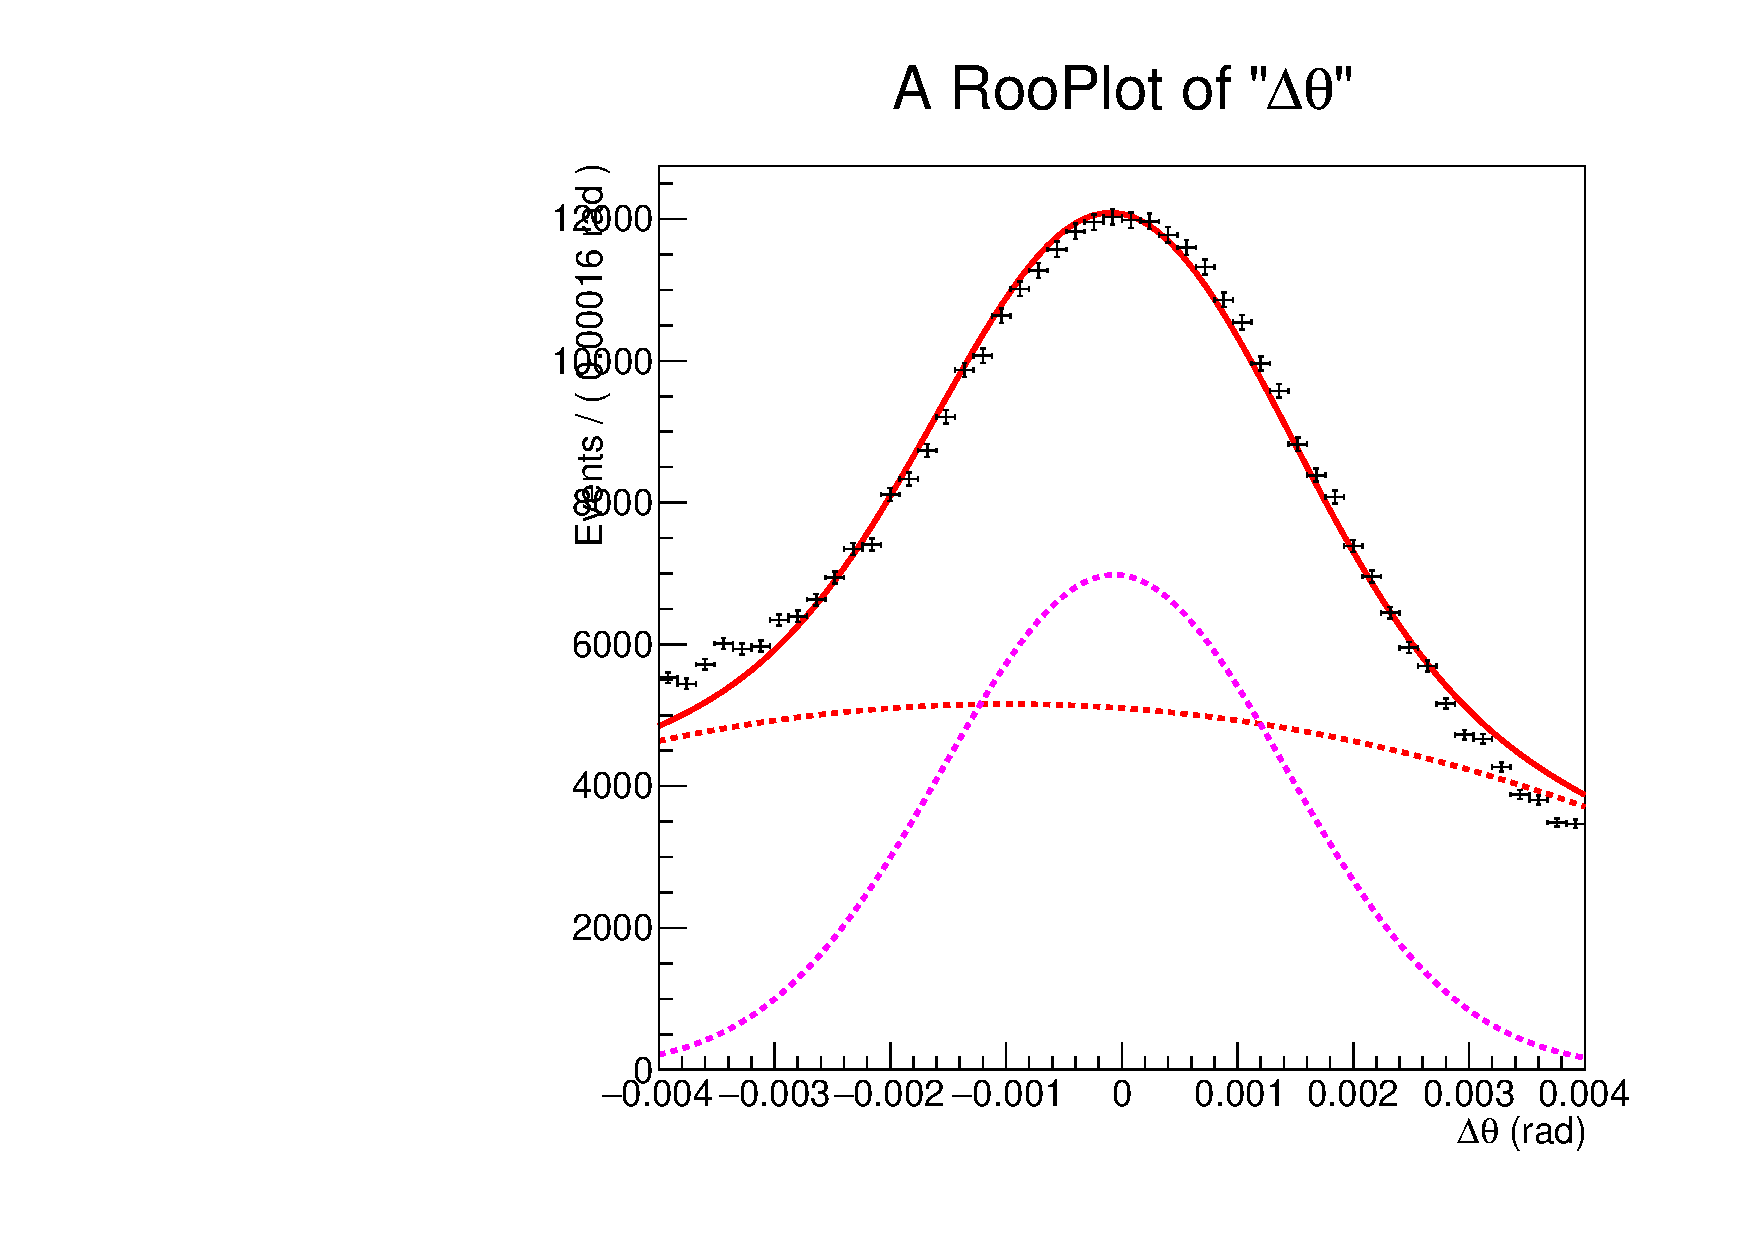
\includegraphics[width=0.7\textwidth]{rootest.pdf}
		\vspace*{-1.cm}
	\end{center}
	\caption{\textit{Example of a fit to the Cherenkov angle resolution distribution for RICH1. Dotted purple line: signal Gaussian, dotted red line: polynomial order 2 background,  solid red line: total function, black points: data points.} }
	\label{fig:fitfunc}
\end{figure}

\section{RICH1}

\subsection{Introduction}
Since each secondary mirror of RICH1 only receives photons from one primary mirror the mirror-pairs are divided into 4 different categories:
\begin{enumerate}
\item secondary mirrors at the outer corners
\item secondary mirrors at the inner corners
\item middle mirror-pairs on bottom and top row
\item middle mirror-pairs on left and right column
\end{enumerate}
The RICH1 mirrors and their categories can be seen in Figure \ref{fig:rich1mirr}. \\
\begin{figure}[!h]
	\vspace*{-0.cm}
	\begin{center}
		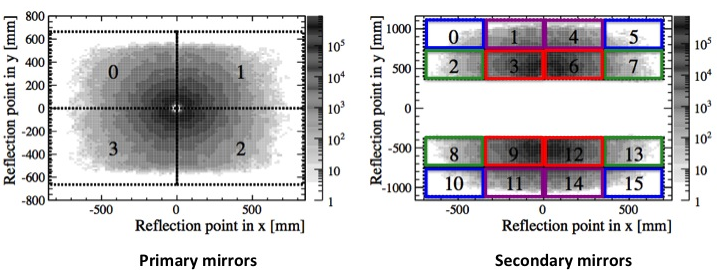
\includegraphics[width=1.\textwidth]{rich1mirrors.png}
		\vspace*{-1.5cm}
	\end{center}
	\caption{\textit{Primary and secondary mirrors of RICH1. Blue: secondary mirrors in category 1 (outer corners), red: secondary mirrors in category 2 (inner corners), purple: secondary mirrors in category 3 (middle in top + bottom row), green secondary mirrors in category 4 (middle in left + right column).}}
	\label{fig:rich1mirr}
\end{figure}
\\
Mirror pairs are denoted by a four-digit number where the first two numbers refer to the primary mirror and the last two to the secondary mirror, e.g. 0001 refers to the pair formed by the top left primary mirror (number 00) and the second secondary mirror in the top row (number 01).\\

\newpage
\subsection{Distribution of the Cherenkov angle resolution}
\label{subsec:rich1dis}
Figure \ref{fig:rich1cherenkov} shows the Cherenkov angle distributions (the projections of the 2D histograms of the Cherenkov angle resolution vs azimuthal angle $\Phi$ onto the Cherenkov angle resolution) for each mirror-pair, grouped into the four categories.\\
\begin{figure}[!h]
	\vspace*{-0.cm}
	\begin{center}
		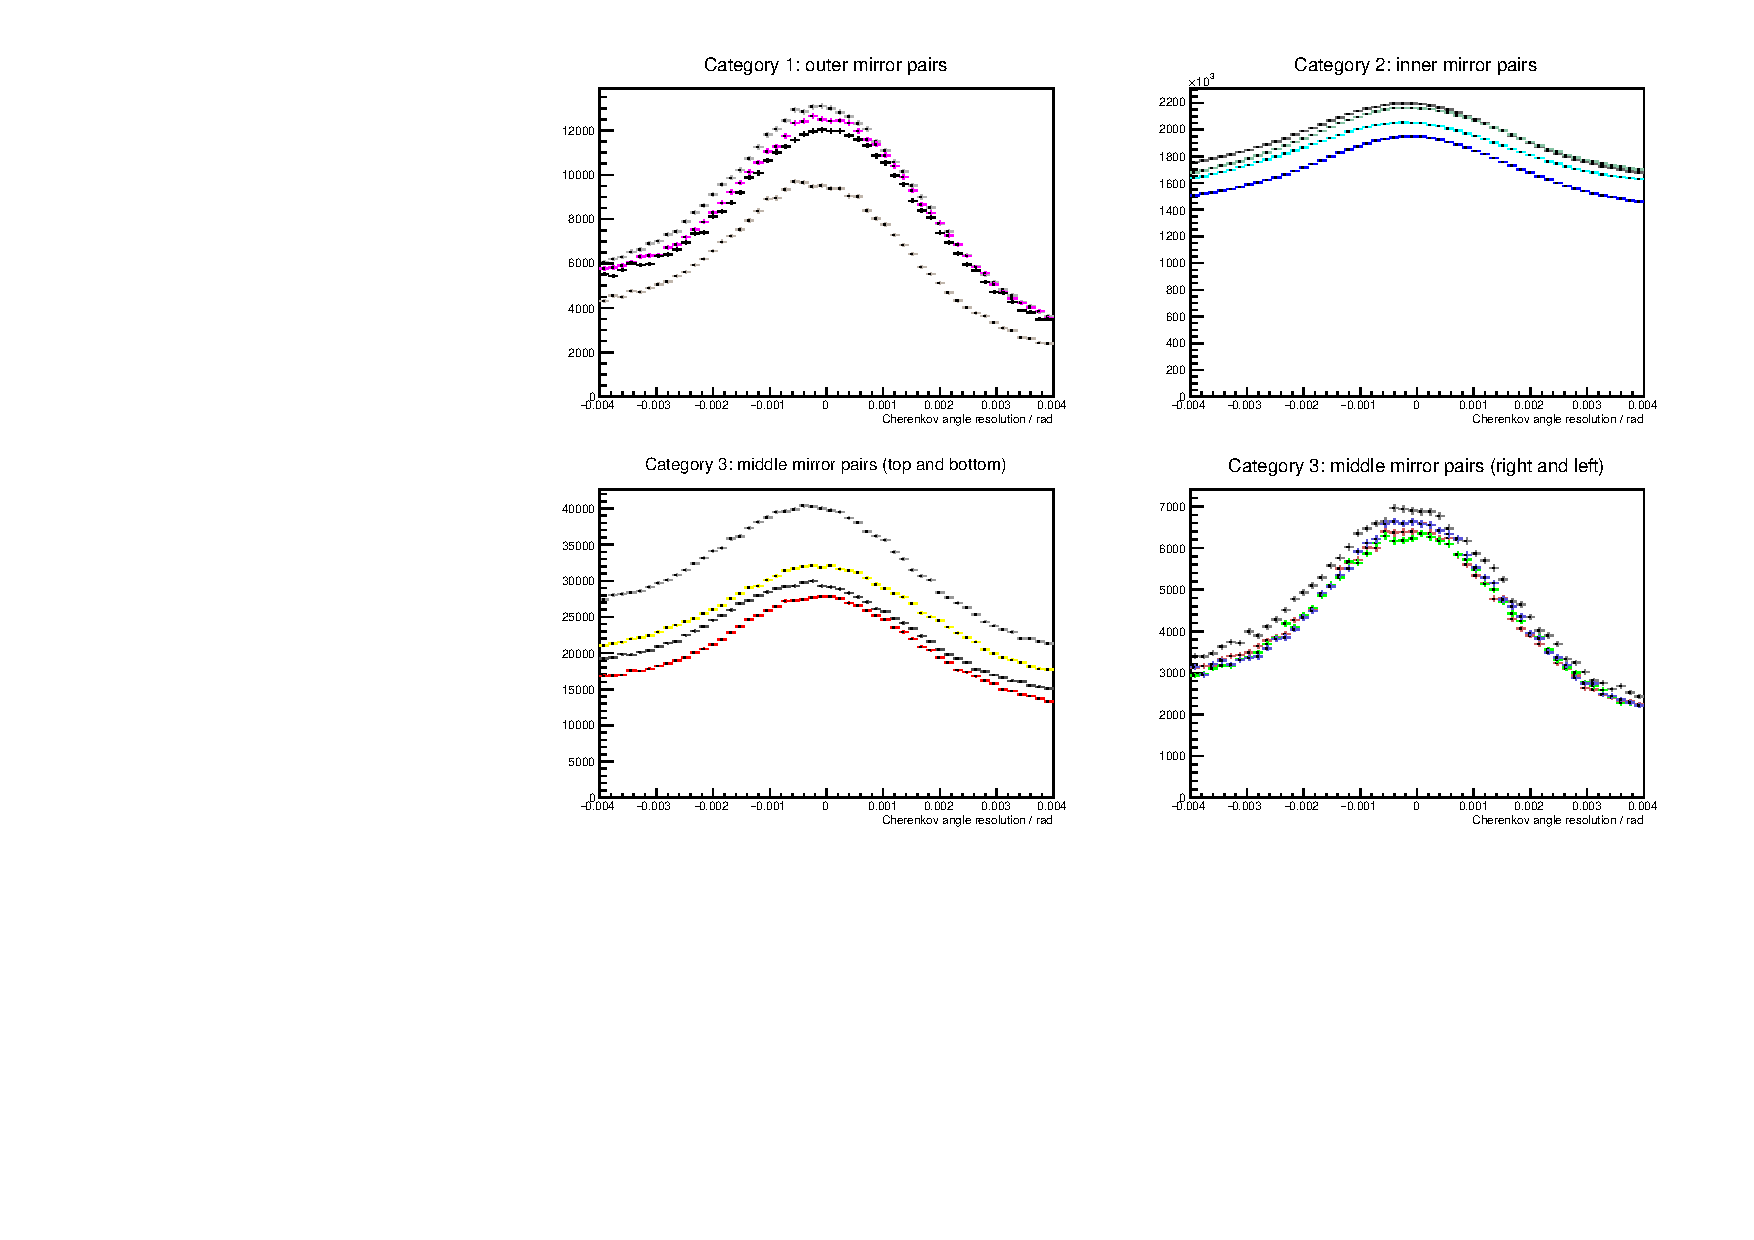
\includegraphics[width=1.\textwidth]{rich1.pdf}
		\vspace*{-1.5cm}
	\end{center}
	\caption{\textit{Distribution of the Cherenkov angle resolution of each mirror pair in RICH1.} Top left: dark grey = 0215, magenta = 0105, black = 0000, light grey = 0310; Top right: grey = 0212, green = 0309, cyan = 0106, blue = 0003; Bottom left: light grey = 0214, yellow = 0104, dark grey = 0311, red = 0001; Bottom right: grey = 0213, blue = 0308, red = 0107, green = 0002. }
	\label{fig:rich1cherenkov}
\end{figure}
The shapes of the Cherenkov angle distributions within each category are consistent. Category 2 has the biggest contribution from bkg while Category 1 has the smallest (see Section \ref{sub:rich1frac} for more). This seems quite intuitive (to me).\\

\newpage
\subsection{Fitted Cherenkov angle resolution by mirror pair}
After the fits on the Cherenkov angle resolution distributions have been performed the fitted Cherenkov angle resolutions (widths of the Gaussian) are plotted for each category in Figure \ref{fig:rich1res}.\\
The fit on the total Cherenkov angle resolution (unambiguous photons only) has also been performed and yields a value of $1.48 \pm 0.01 \ mrad$.\\

\begin{figure}[!h]
	\vspace*{-0.cm}
	\begin{center}
		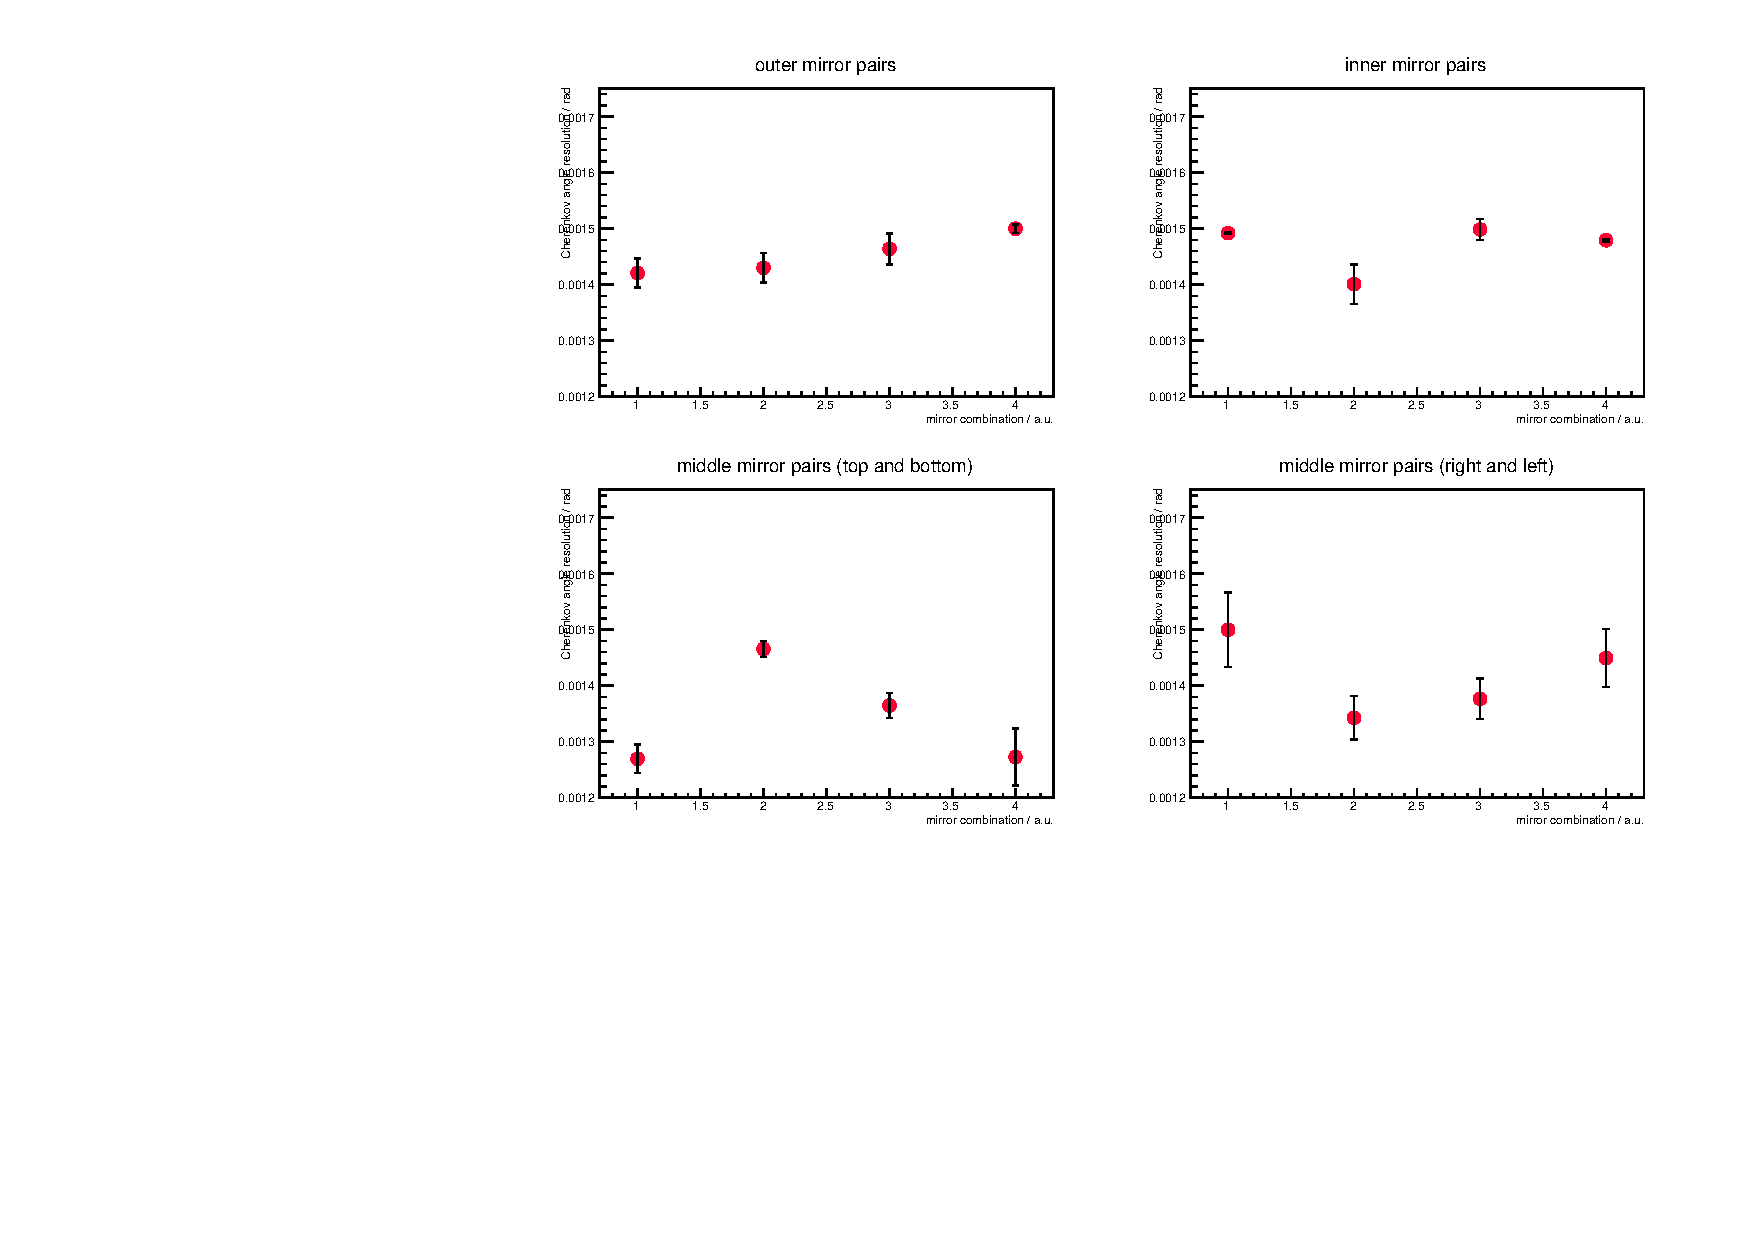
\includegraphics[width=1.\textwidth]{res_rich1.pdf}
		\vspace*{-1.5cm}
	\end{center}
	\caption{\textit{Cherenkov angle resolution of each mirror pair in RICH1 for the four different categories (note that the range of the y-axis is the same for all four plots).} Top left: 1 = 0000, 2 = 0105, 3 = 0310, 4 = 0215; Top right: 1 = 0003, 2 = 0106, 3 = 0309, 4 = 0212 ; Bottom left: 1 = 0001, 2 = 0104, 3 = 0311, 4 = 0214; Bottom right:1 = 0002, 2 = 0107, 3 = 0308, 4 = 0213. }
	\label{fig:rich1res}
\end{figure}
\\ 
The resolutions seem to roughly agree with each other within each category and amongst the categories. The amount of bkg does not affect the Cherenkov angle resolution.\\


\newpage
\subsection{Fraction of signal photons}
\label{sub:rich1frac}
Figure \ref{fig:rich1sigfrac} shows the number of fraction of signal photons as obtained from the fit for each category.
\begin{equation}
fraction = \frac{N^{sig}_{\gamma}}{N^{sig}_{\gamma} + N^{bkg}_{\gamma}}
\end{equation}
where $N^{sig}_{\gamma}$ and $N^{bkg}_{\gamma}$ have been determined by the fit.\\
\begin{figure}[!h]
	\vspace*{-0.cm}
	\begin{center}
		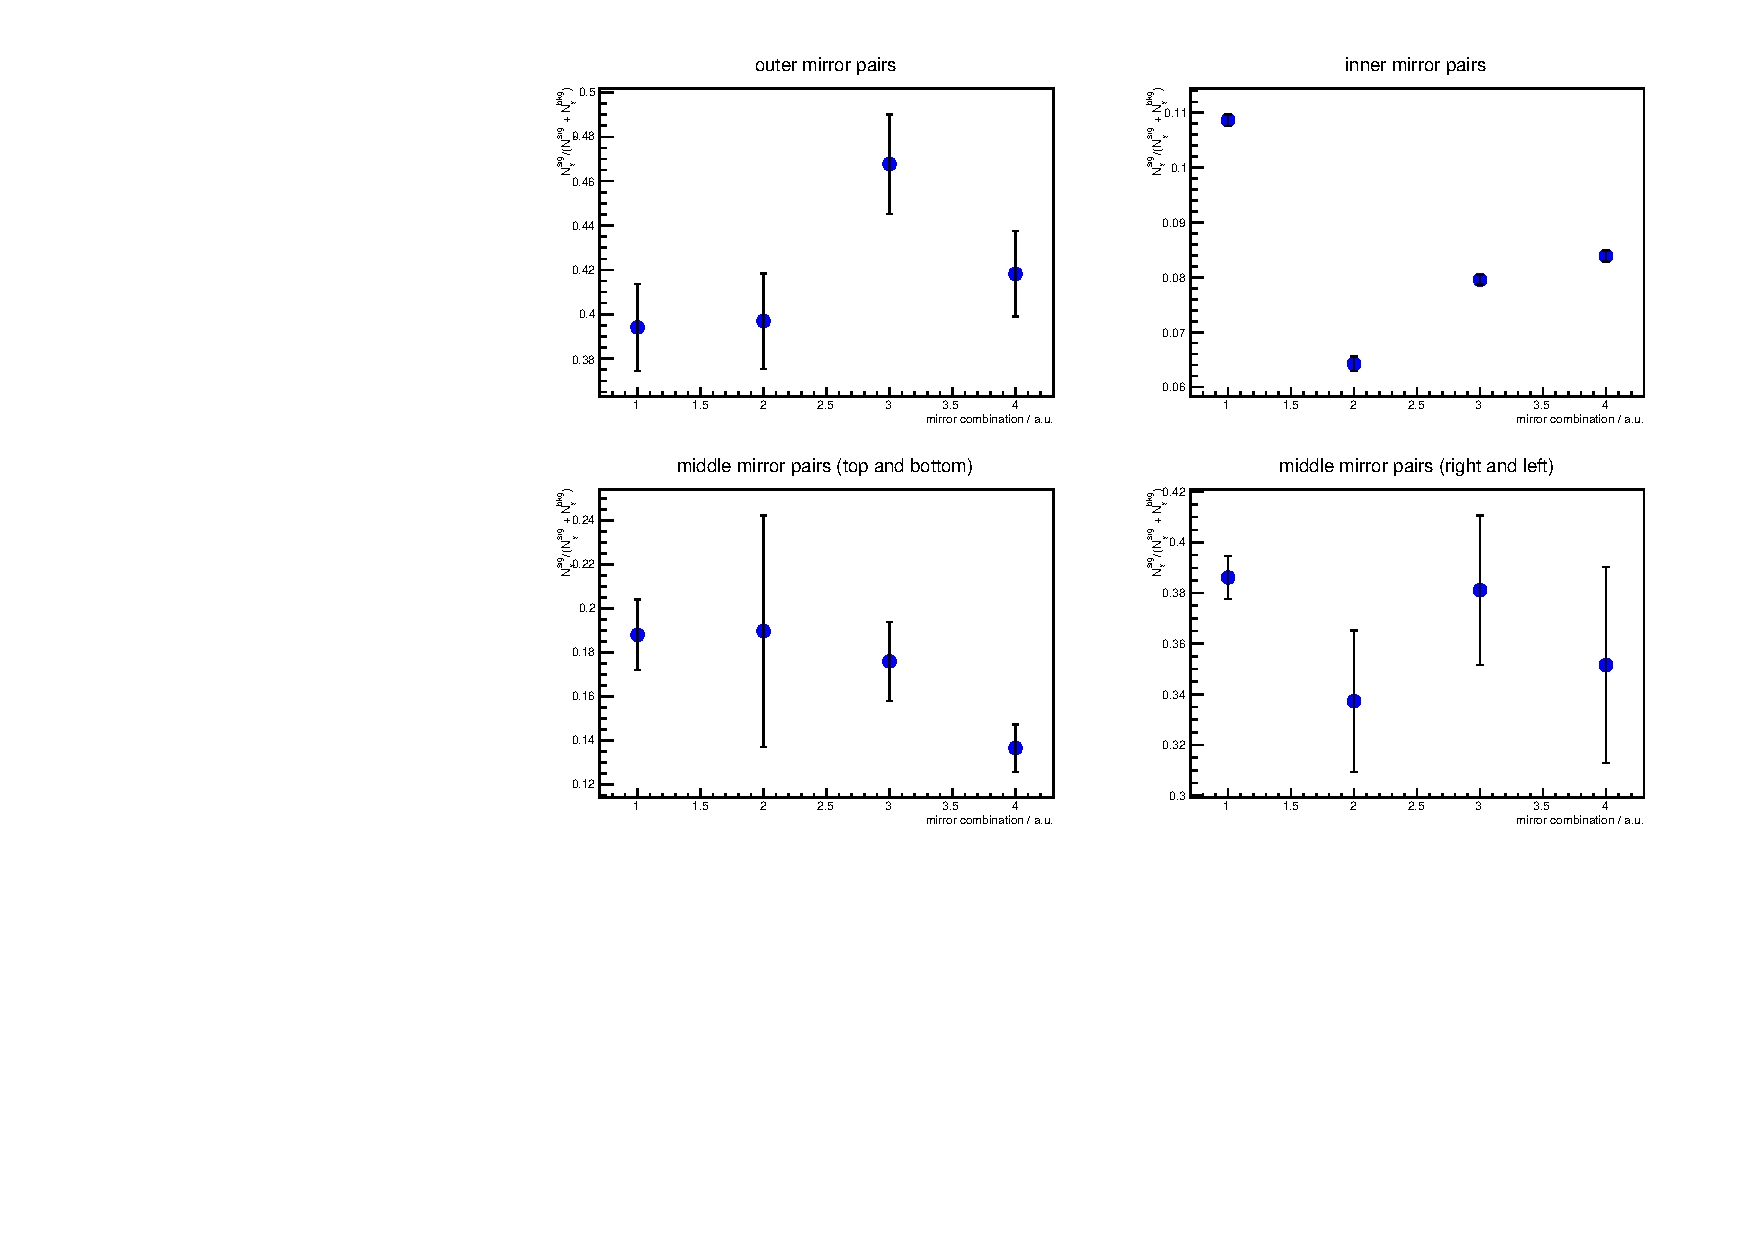
\includegraphics[width=1.\textwidth]{sigfrac_rich1.pdf}
		\vspace*{-1.5cm}
	\end{center}
	\caption{\textit{Fraction of signal photons as determined by the fit for each mirror pair in RICH1 for the four different categories. The error in the number of entries N is taken to be $\sqrt{N}$.} Top left: 1 = 0000, 2 = 0105, 3 = 0310, 4 = 0215; Top right: 1 = 0003, 2 = 0106, 3 = 0309, 4 = 0212 ; Bottom left: 1 = 0001, 2 = 0104, 3 = 0311, 4 = 0214; Bottom right:1 = 0002, 2 = 0107, 3 = 0308, 4 = 0213. }
	\label{fig:rich1sigfrac}
\end{figure}

Category 1 has the greatest contribution from signal photons while Category 2 has the smallest. For all categories except the \textit{inner mirror pairs} the values for the signal fraction agree within a category.\\
\textbf{Is the discrepancy within Category 2 (inner mirror pairs) problematic?}
\newpage




\subsection{Entries in 2D histograms by mirror pair}
As can be seen in Section \ref{subsec:rich1dis} the total amount of entries in the 2D histograms per mirror pair varies even inside a given category. Figure \ref{fig:rich1entries} shows the number of entries for each mirror pair for each category.
\begin{figure}[!h]
	\vspace*{-0.5cm}
	\begin{center}
		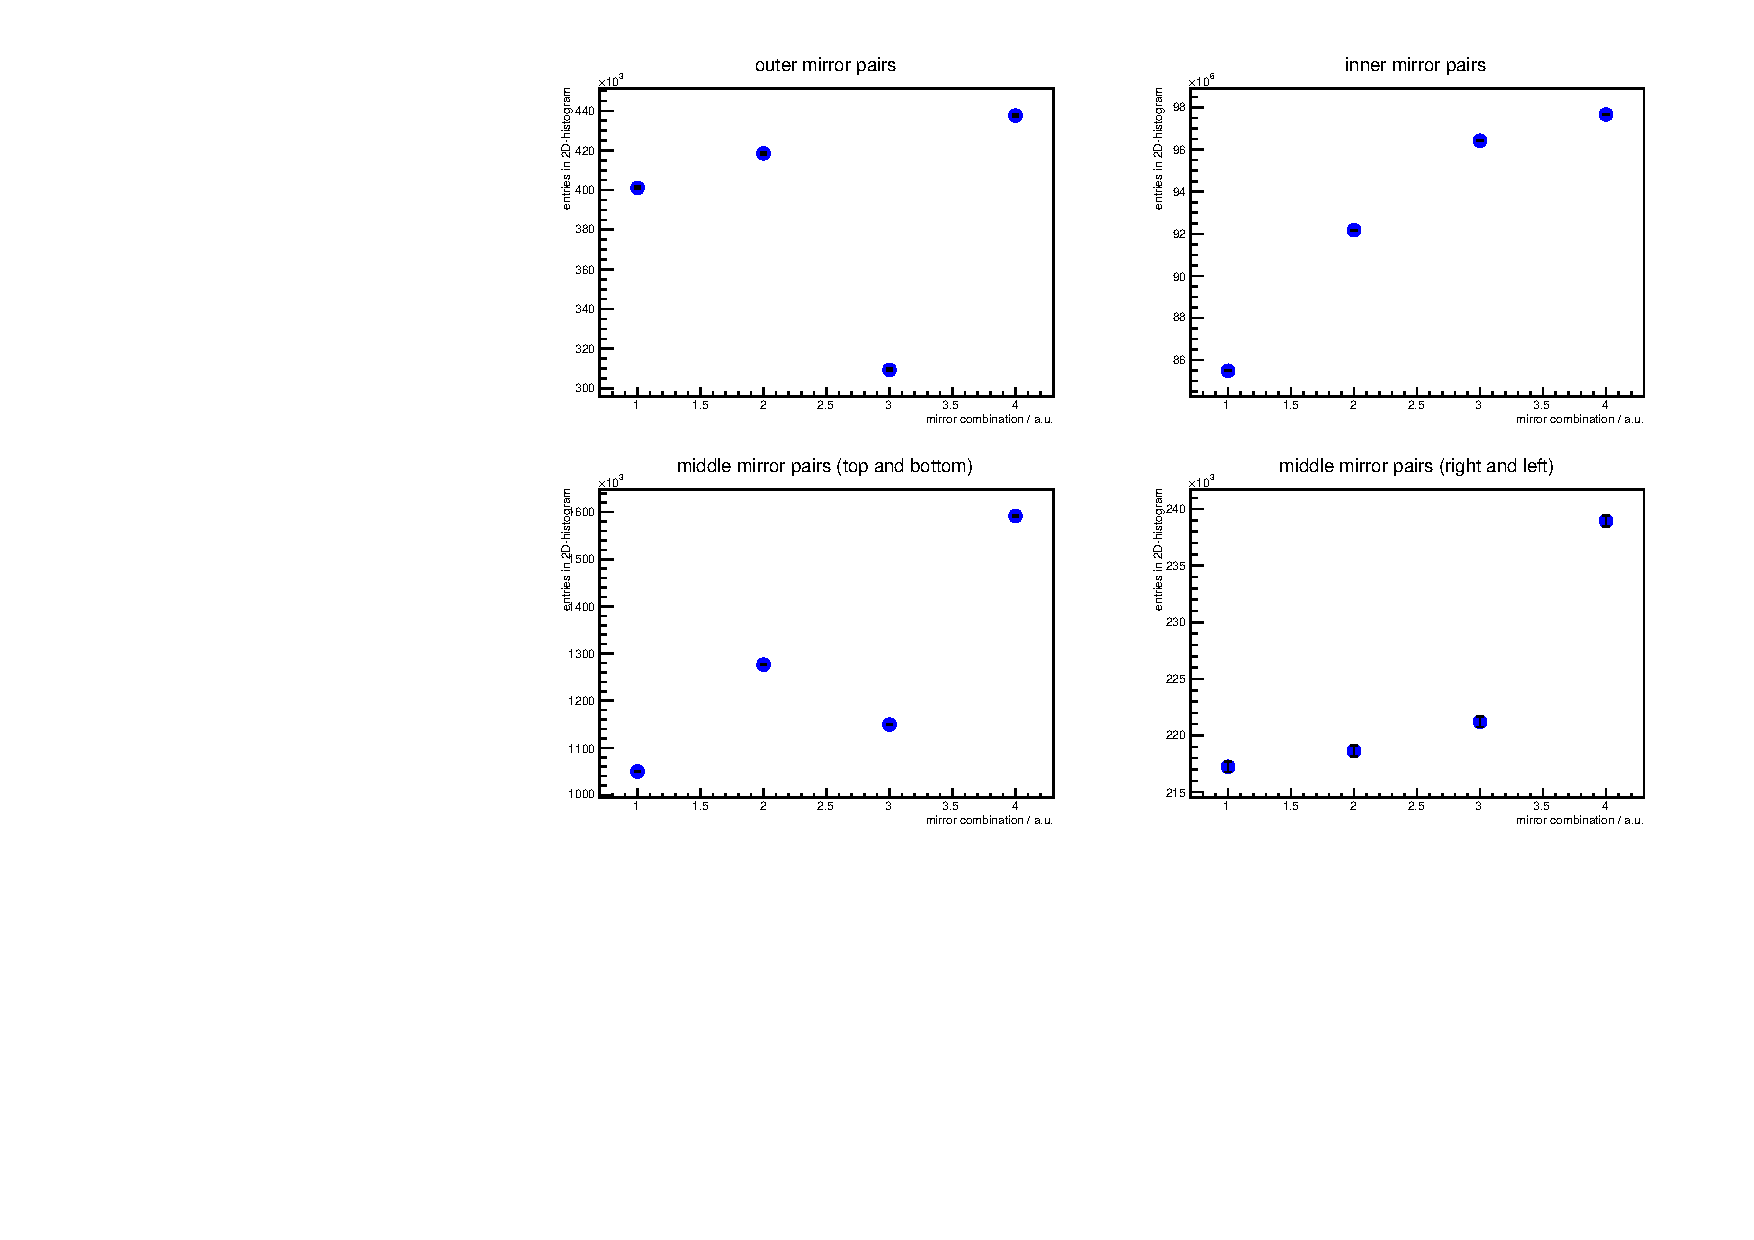
\includegraphics[width=1.\textwidth]{entries_rich1.pdf}
		\vspace*{-1.5cm}
	\end{center}
	\caption{\textit{Entries in histogram for each mirror pair in RICH1 for the four different categories. The error in the number of entries N is taken to be $\sqrt{N}$.} Top left: 1 = 0000, 2 = 0105, 3 = 0310, 4 = 0215; Top right: 1 = 0003, 2 = 0106, 3 = 0309, 4 = 0212 ; Bottom left: 1 = 0001, 2 = 0104, 3 = 0311, 4 = 0214; Bottom right:1 = 0002, 2 = 0107, 3 = 0308, 4 = 0213. }
	\label{fig:rich1entries}
\end{figure}
For clearer comparison the number of entries per histogram is also plotted normalised to the first mirror-pair in each category respectively in Figure \ref{fig:rich1relentries}.
\begin{figure}[!h]
	\vspace*{-1.5cm}
	\begin{center}
		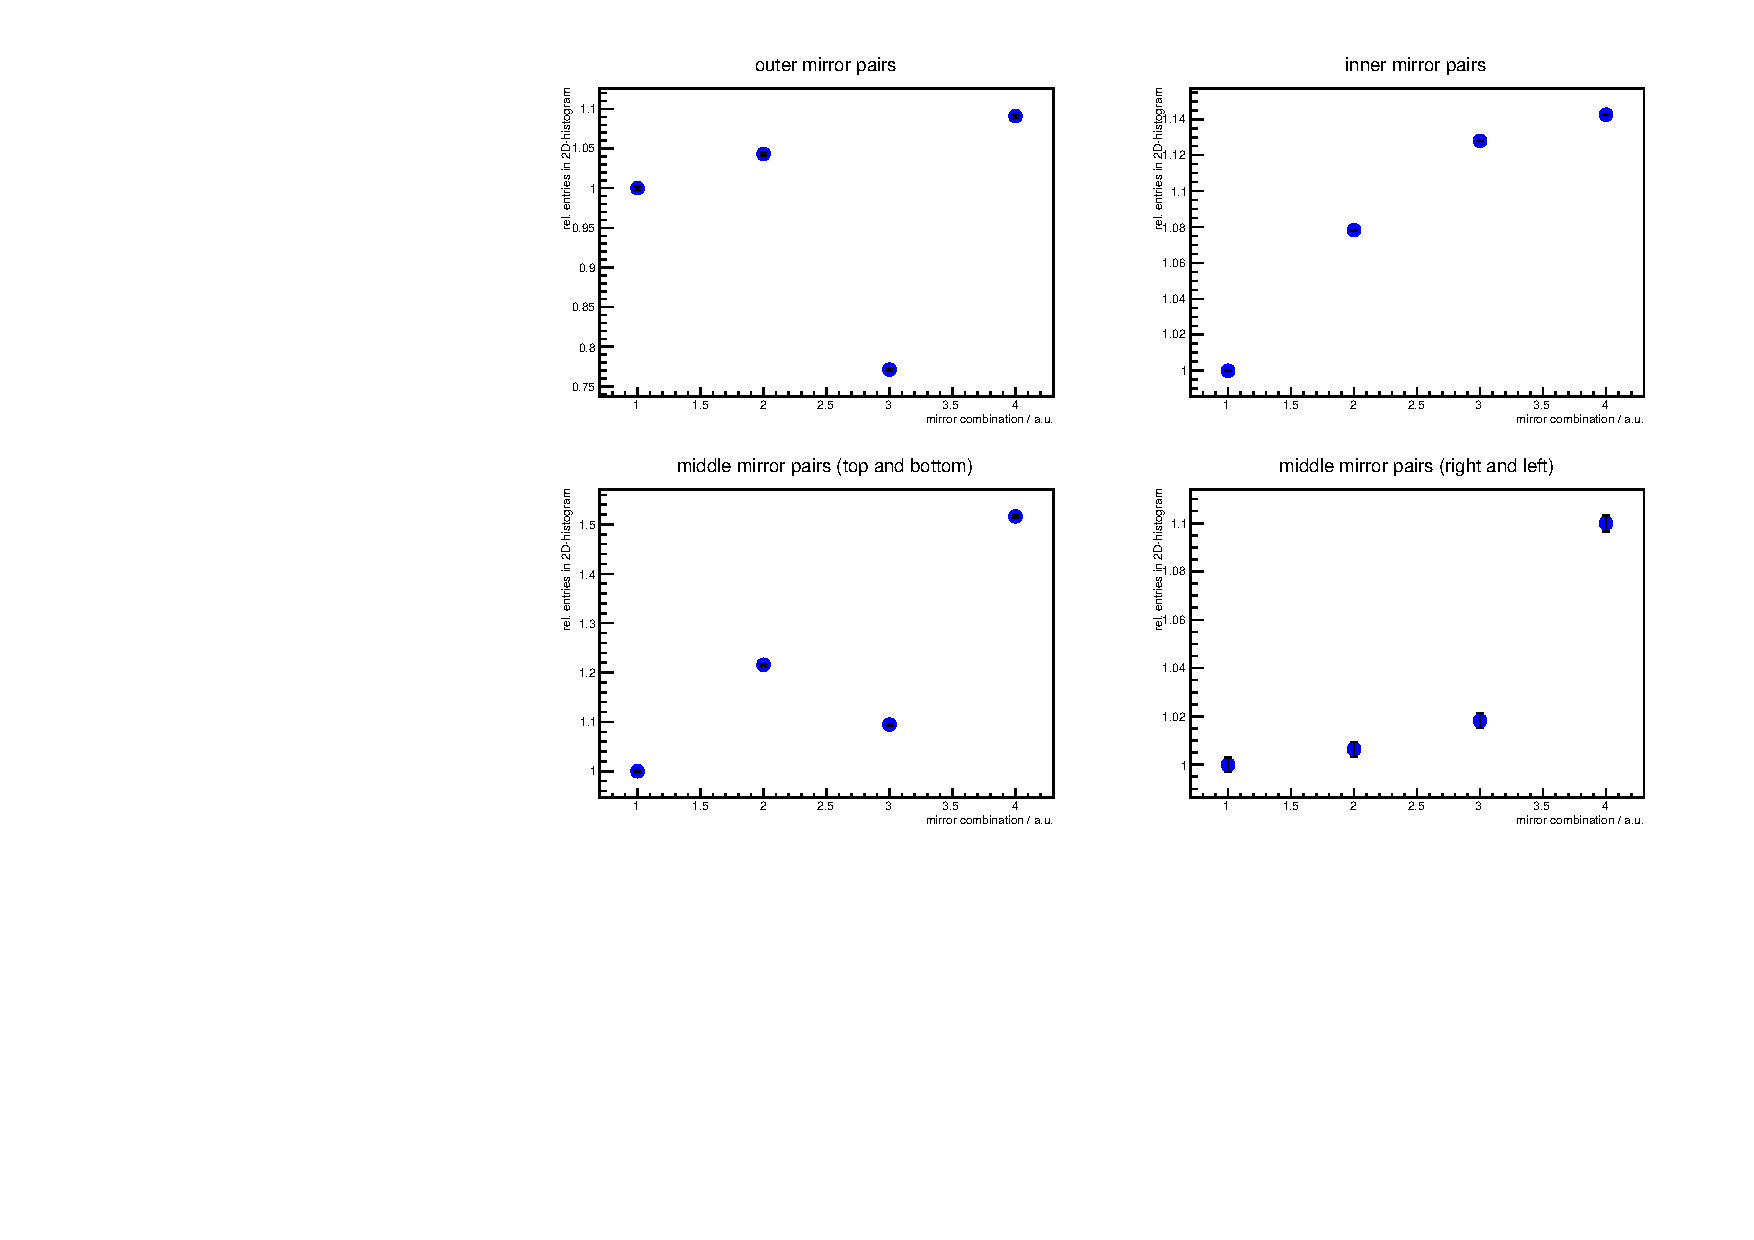
\includegraphics[width=1.\textwidth]{relentries_rich1.pdf}
		\vspace*{-1.5cm}
	\end{center}
	\caption{\textit{Entries in histogram for each mirror pair in RICH1 normalised to the first mirror-pair in each category respectively.} }
	\label{fig:rich1relentries}
\end{figure}

The numbers of entries within each category vary much more than the statical fluctuation. This might be due to a asymmetry in the HLT line. \textbf{Could this be explained otherwise?}

\clearpage

\section{RICH2}
The study was performed on the histograms made in the last iteration of the fully converged alignment from 19.07.2015 which is at present time the latest RICH2 alignment.\\
\\ 
\subsection{Introduction}
In RICH2 one given primary mirror can reflect onto several secondary mirrors and one given secondary mirror can receive photons from several primary mirrors. The primary and secondary mirrors of RICH2 are shown in Figure \ref{fig:rich2mirr}. The mirror-pairs for the left side of the RICH2 used in the alignment are shown in Figure \ref{fig:rich2combis}, the right side is equivalent. 
\begin{figure}[!h]
	\vspace*{-0.cm}
	\begin{center}
		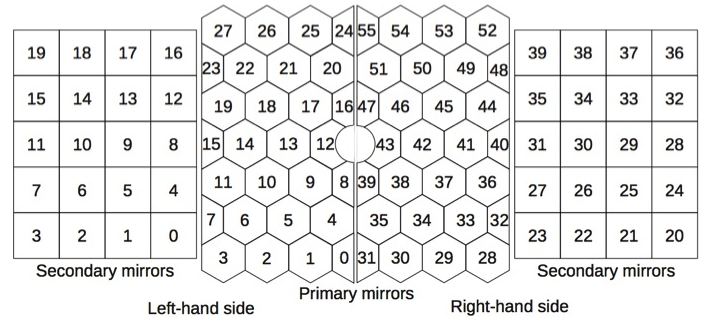
\includegraphics[width=1.\textwidth]{rich2mirrors.png}
		\vspace*{-1.cm}
	\end{center}
	\caption{\textit{Primary and secondary mirrors of RICH2.}}
	\label{fig:rich2mirr}
\end{figure}

\begin{figure}[!h]
	\vspace*{-0.cm}
	\begin{center}
		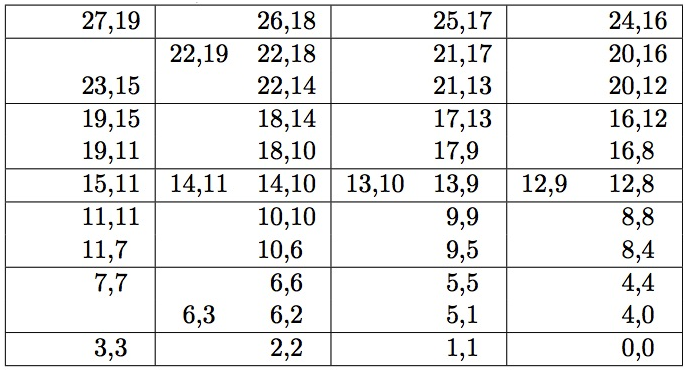
\includegraphics[width=0.7\textwidth]{rich2combis.png}
		\vspace*{-0.5cm}
	\end{center}
	\caption{\textit{Mirror combinations of the left side of RICH2 used in the alignment procedure.}}
	\label{fig:rich2combis}
\end{figure}

Mirror pairs are denoted by a four-digit number where the first two numbers refer to the primary mirror and the last two to the secondary mirror, e.g. 2820 refers to the pair formed by the very bottom right primary mirror (number 28) and the very bottom right secondary mirror (number 20).\\

\subsection{Fitted Cherenkov angle resolution by mirror pair}
After the fits on the Cherenkov angle resolution distributions have been performed the fitted Cherenkov angle resolutions (widths of the Gaussian) are plotted for each mirror-pair in Figure \ref{fig:rich2res}.\\
The fit on the total Cherenkov angle resolution (unambiguous photons only) has also been performed and yields a value of $0.591 \pm 0.000 \ mrad$.
\begin{figure}[!h]
	\vspace*{-0.cm}
	\begin{center}
		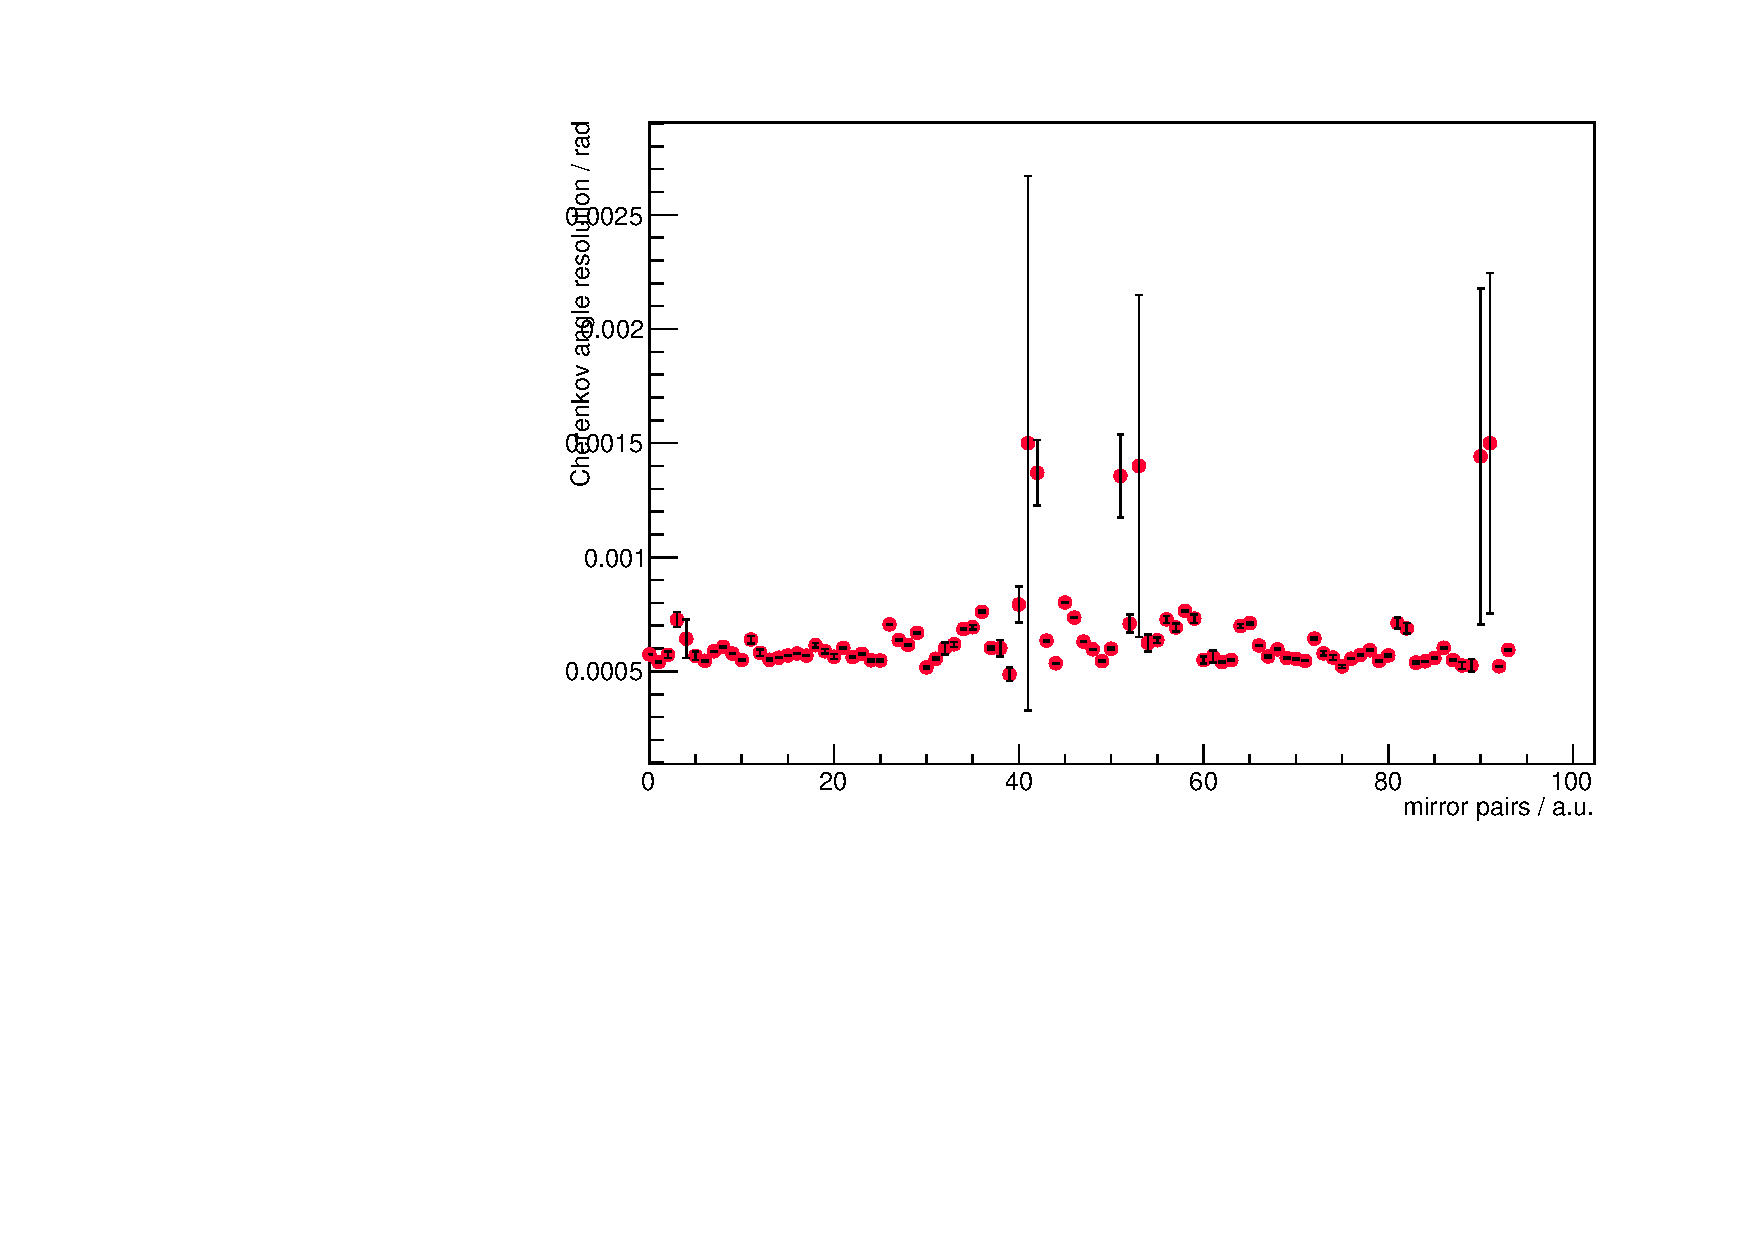
\includegraphics[width=1.\textwidth]{resdis_rich2.pdf}
		\vspace*{-1.5cm}
	\end{center}
	\caption{\textit{Cherenkov angle resolution of each mirror-pair in RICH2 used in the alignment.} \textbf{Note: Six mirror-pairs (1411, 1410, 4129, 4028, 3123, 3022) have relatively big values for the resolution (> 0.1mrad), this is only due to the fits failing as can be seen in Figures \ref{fig:rich2p4}, \ref{fig:rich2p5} and \ref{fig:rich2p8}.}}
	\label{fig:rich2res}
\end{figure}
Like for RICH1 the Cherenkov angle resolution is independent from the mirror-pair.\\

\subsection{Fraction of signal photons}
Figure \ref{fig:rich2sigfrac} shows the number of fraction of signal photons as obtained from the fit for each category.
\begin{equation}
fraction = \frac{N^{sig}_{\gamma}}{N^{sig}_{\gamma} + N^{bkg}_{\gamma}}
\end{equation}
where $N^{sig}_{\gamma}$ and $N^{bkg}_{\gamma}$ have been determined by the fit.\\
\begin{figure}[!h]
	\vspace*{-0.cm}
	\begin{center}
		\subfigure{ 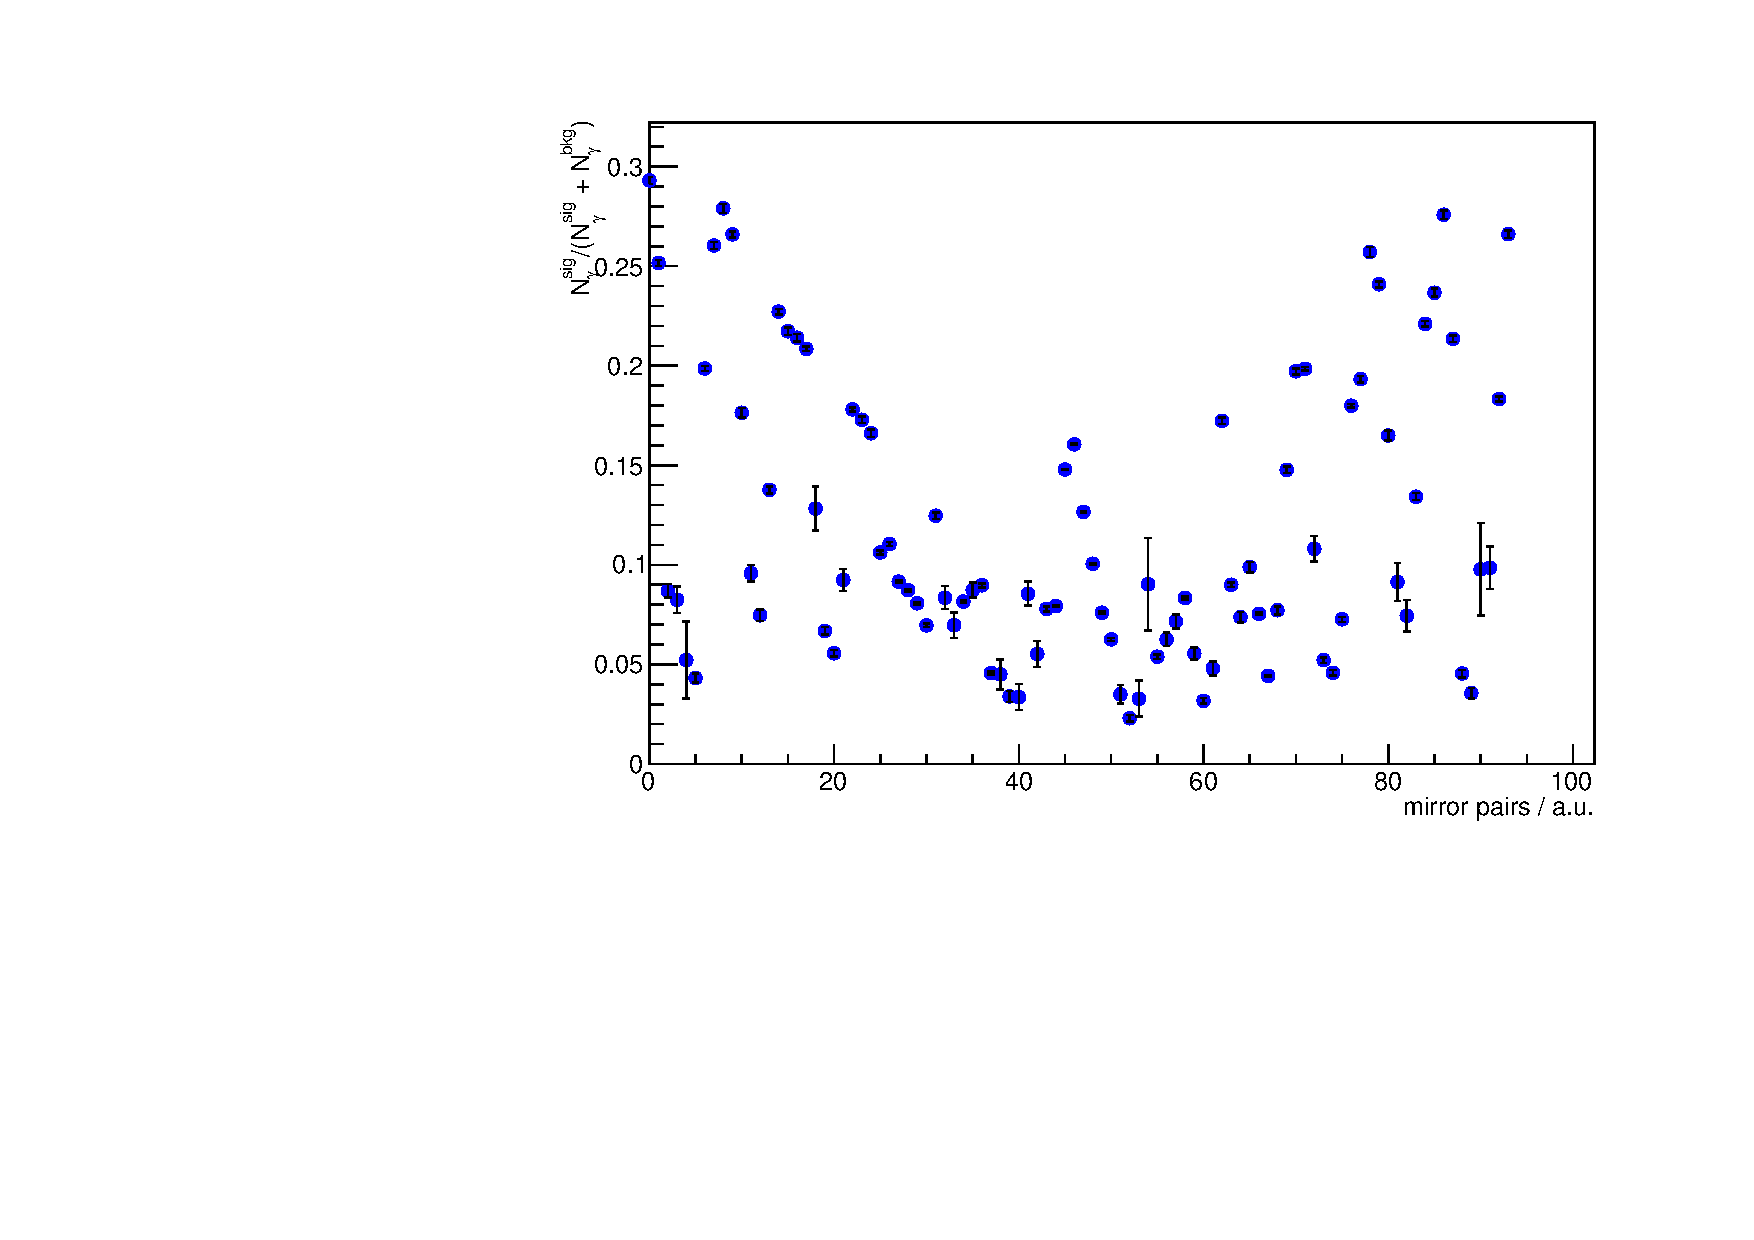
\includegraphics[width=0.48 \textwidth] {sigfrac_rich2.pdf}}
		\subfigure{ 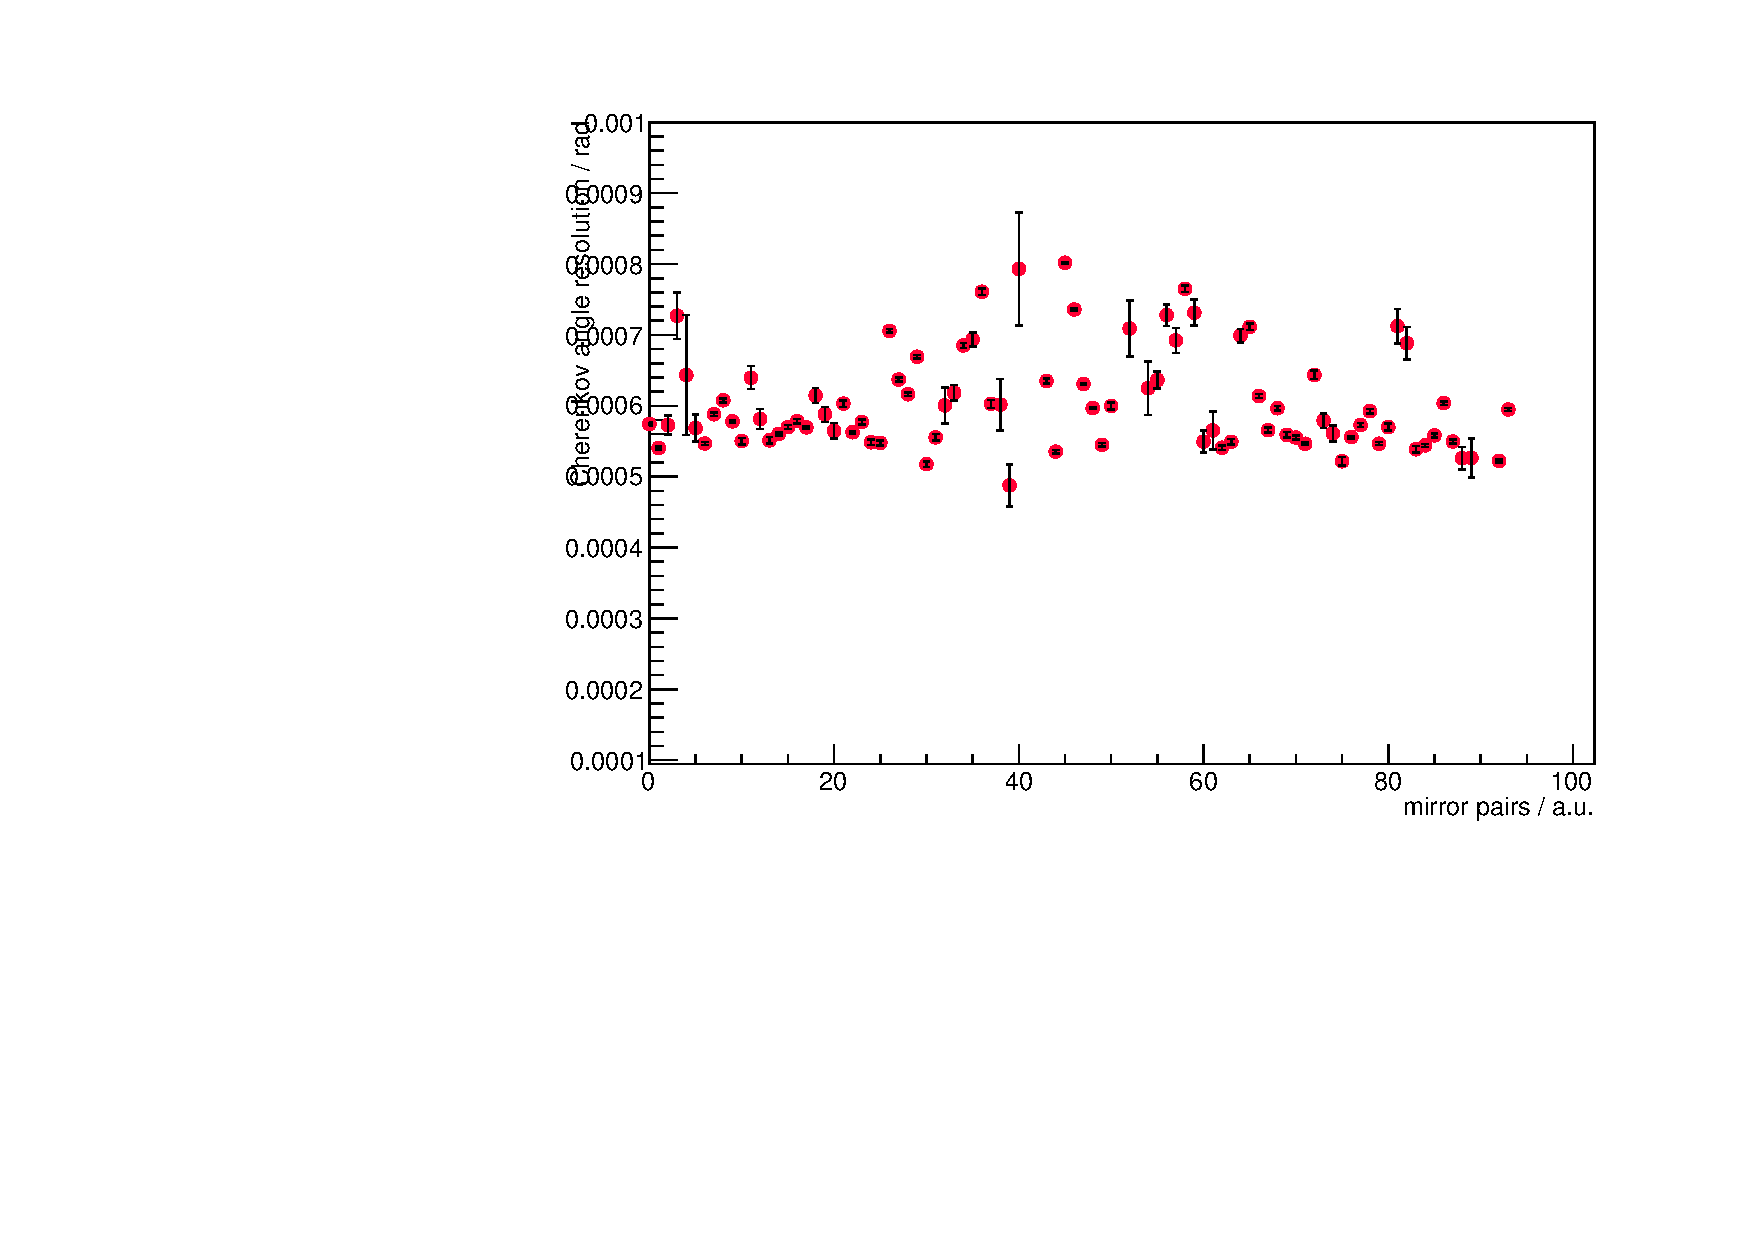
\includegraphics[width=0.48 \textwidth] {resdis_rich2ZOOM.pdf}}
		\vspace*{-0.5cm}
	\end{center}
	\caption{\textit{Left: Fraction of signal photons as determined by the fit for each mirror-pair in RICH2. Right: Cherenkov angle resolution for each mirror-pair with successful fit.}}
	\label{fig:rich2sigfrac}
\end{figure}
As can be verified in Figures \ref{fig:rich2p1} - \ref{fig:rich2p8} the mirror-pairs with high signal fractions are those on the outer corners of RICH2 and those on top and bottom. The mirror-combinations with the lowest signal contribution are not those closest to the beampipe but rather those that lay horizontally in the middle of RICH2.\\
As can be seen by comparing both plots in Figure \ref{fig:rich2sigfrac} the Cherenkov angle resolution does not depend on the signal fraction.\\

\subsection{Entries in 2D histograms by mirror pair}
Figure \ref{fig:rich2entries} shows the number of entries in the 2D histograms of the Cherenkov angle resolution vs azimuthal angle $\Phi$ for each mirror-pair.\\
\begin{figure}[!h]
\begin{center}
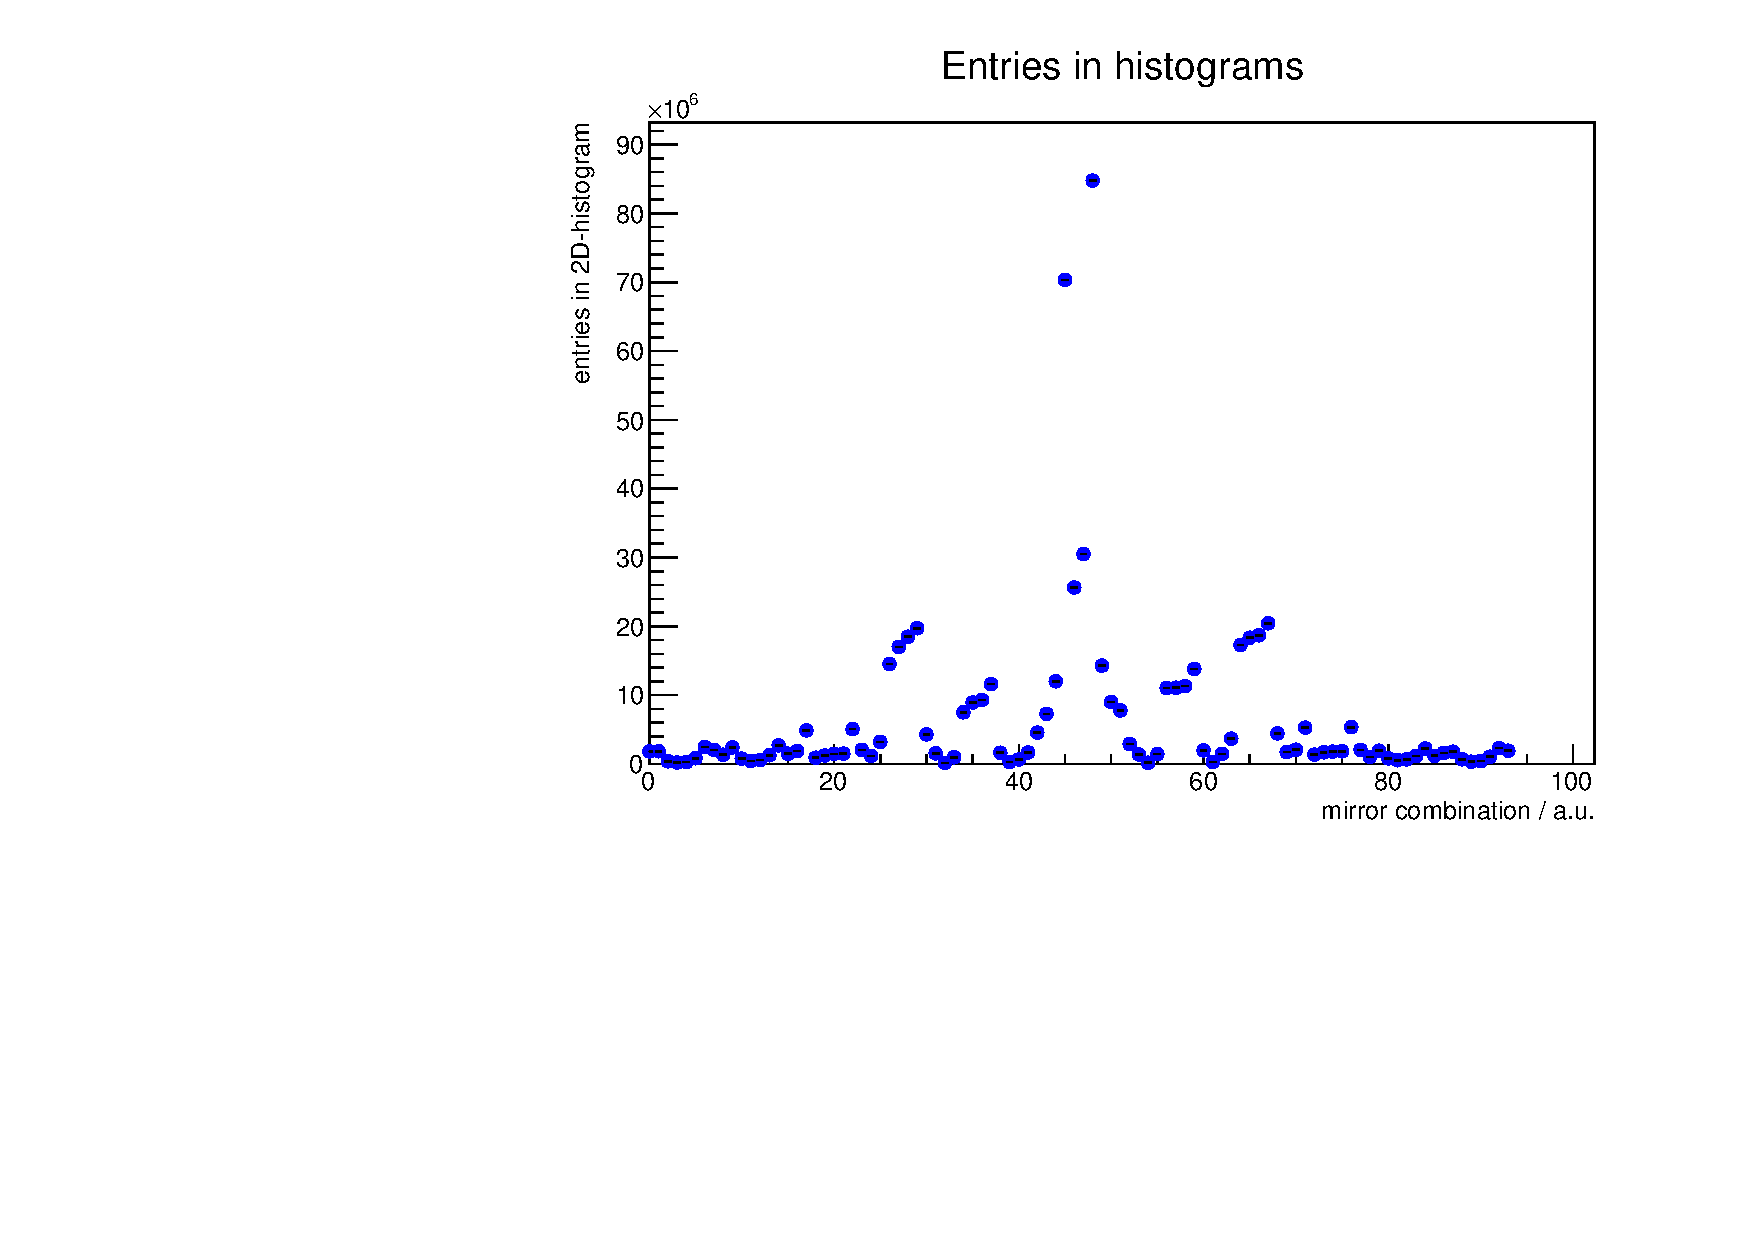
\includegraphics[width= 0.7\textwidth] {entries_rich2.pdf}
\end{center}
\caption{\textit{Entries in histogram for each mirror-pair in RICH2. The error in the number of entries N is taken to be $\sqrt{N}$.}}
\label{fig:rich2entries}
\end{figure}
The mirror-pairs with visibly many entries (more than $15 \cdot 10^{6}$ entries) are as expected those closest to the beampipe.\\



\section{Every single Cherenkov angle resolution fit}
\subsection{RICH1}
\begin{figure}[!h]
	\vspace*{-0.cm}
	\begin{center}
		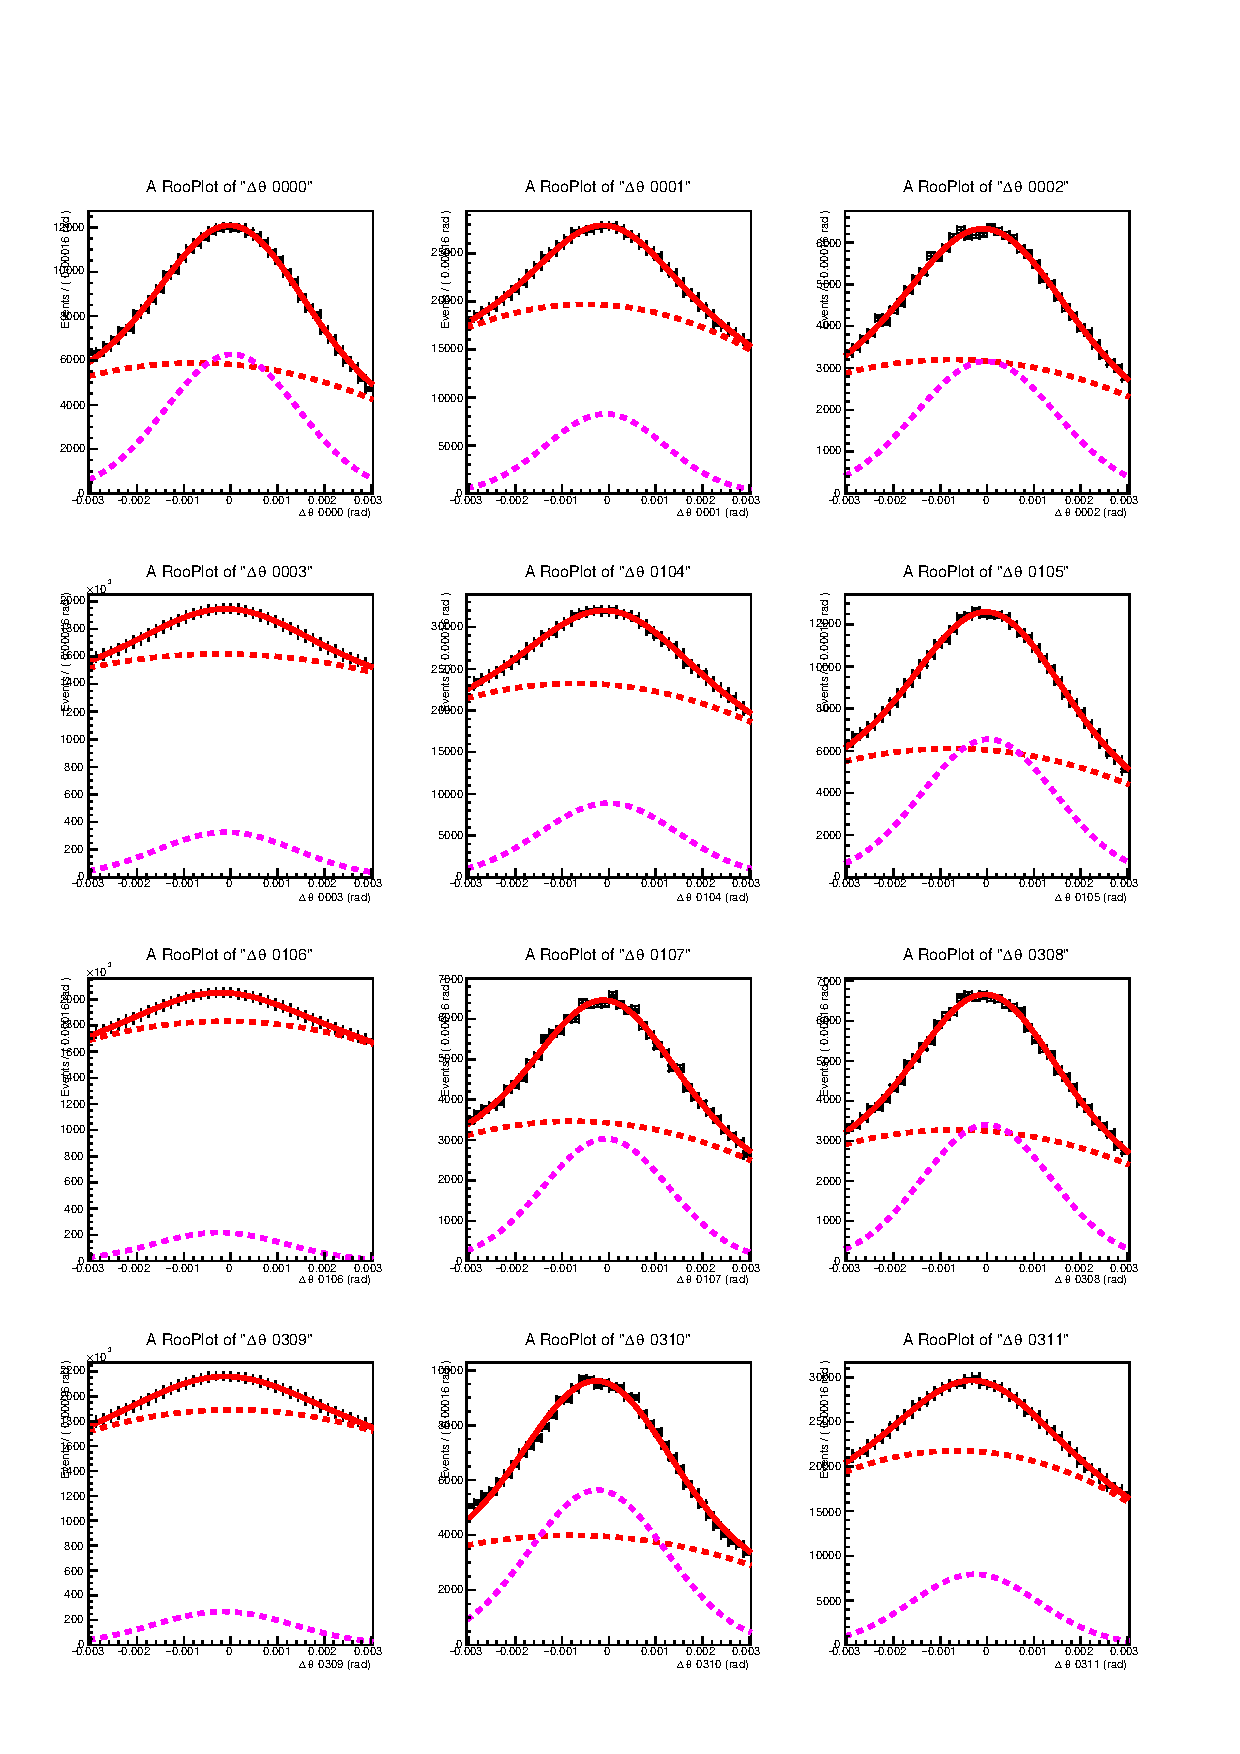
\includegraphics[width=1.\textwidth]{rich1_p1.pdf}
		\vspace*{-1.5cm}
	\end{center}
	\caption{\textit{Fit to the Cherenkov angle resolution distribution for RICH1 mirror-pairs.}}
	\label{fig:rich1p1}
\end{figure}
\clearpage
\begin{figure}[!h]
	\vspace*{-0.cm}
	\begin{center}
		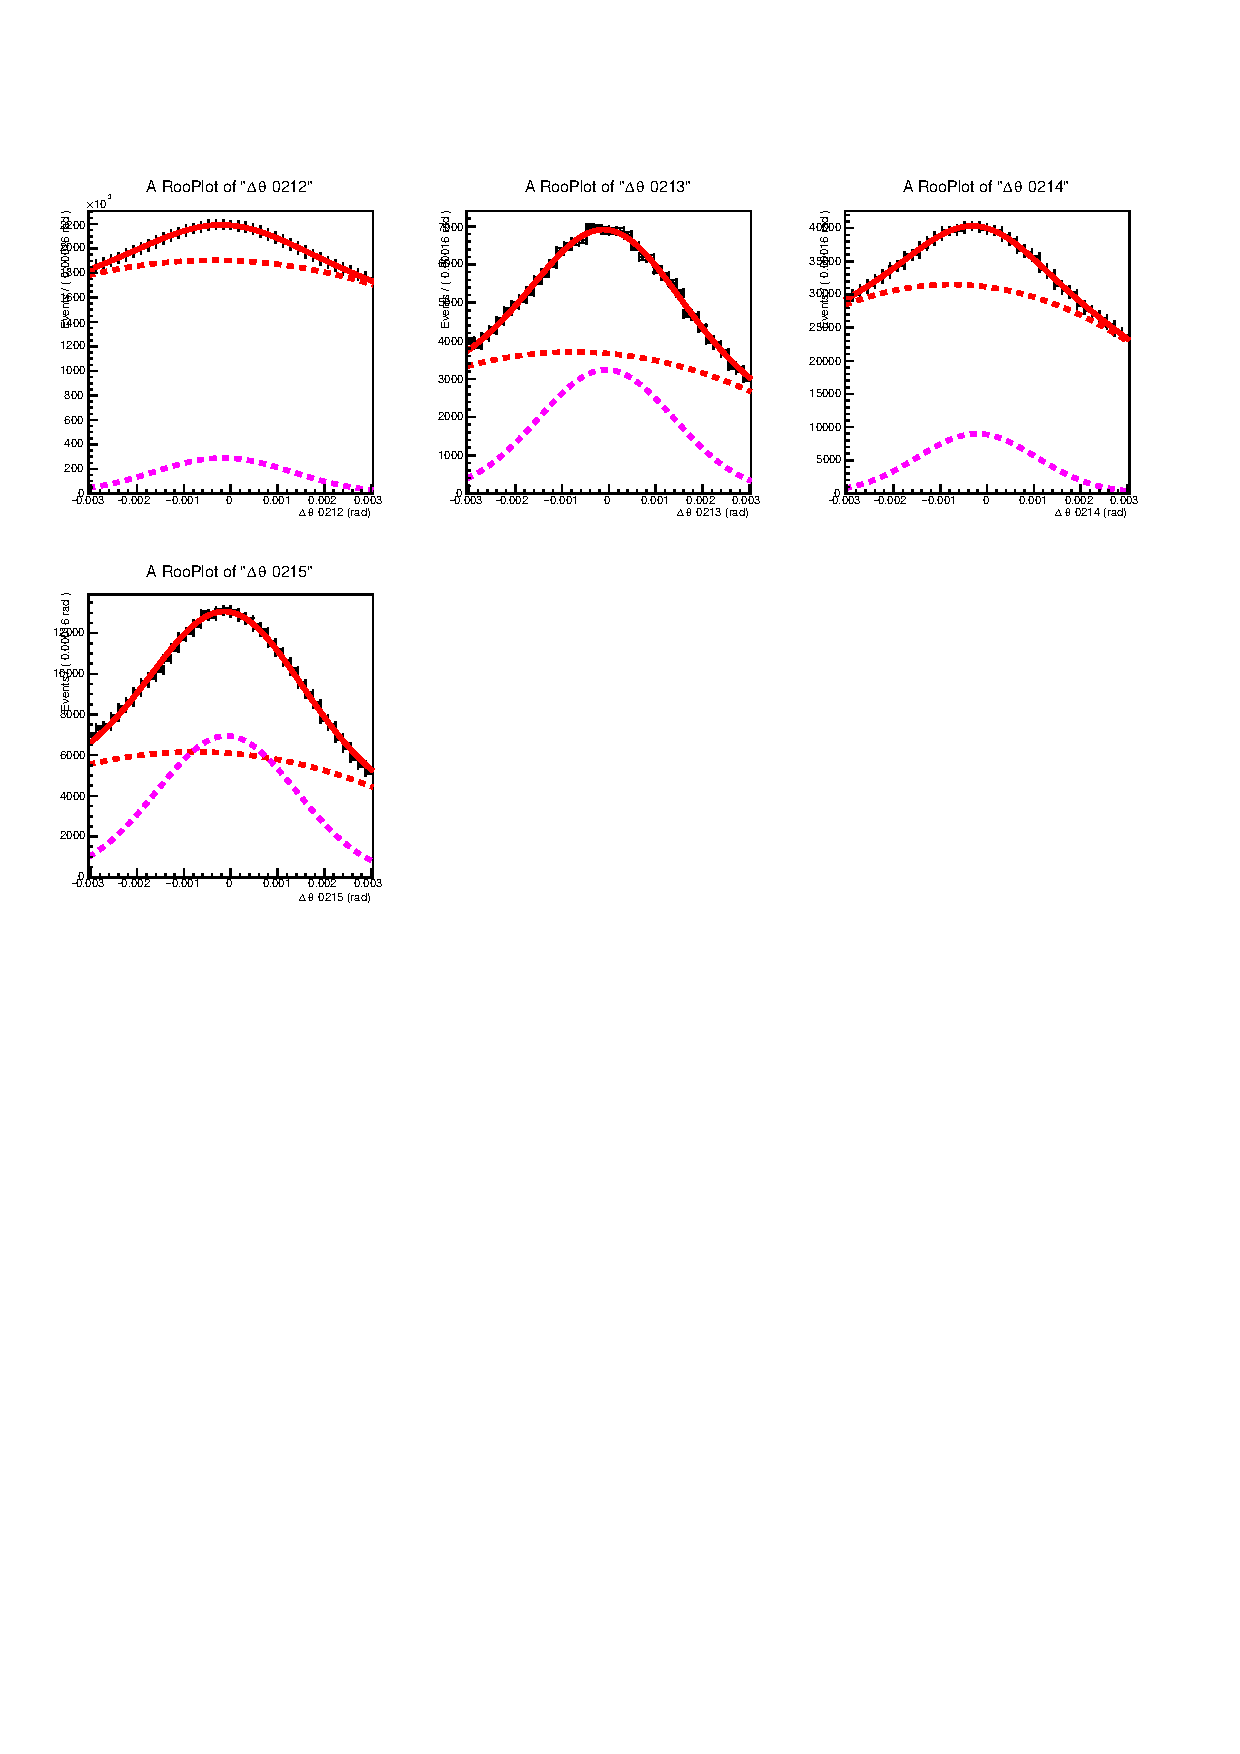
\includegraphics[width=1.\textwidth]{rich1_p2.pdf}
		\vspace*{-1.5cm}
	\end{center}
	\caption{\textit{Fit to the Cherenkov angle resolution distribution for RICH1 mirror-pairs.}}
	\label{fig:rich1p2}
\end{figure}
\clearpage
\subsection{RICH2}
\begin{figure}[!h]
	\vspace*{-0.cm}
	\begin{center}
		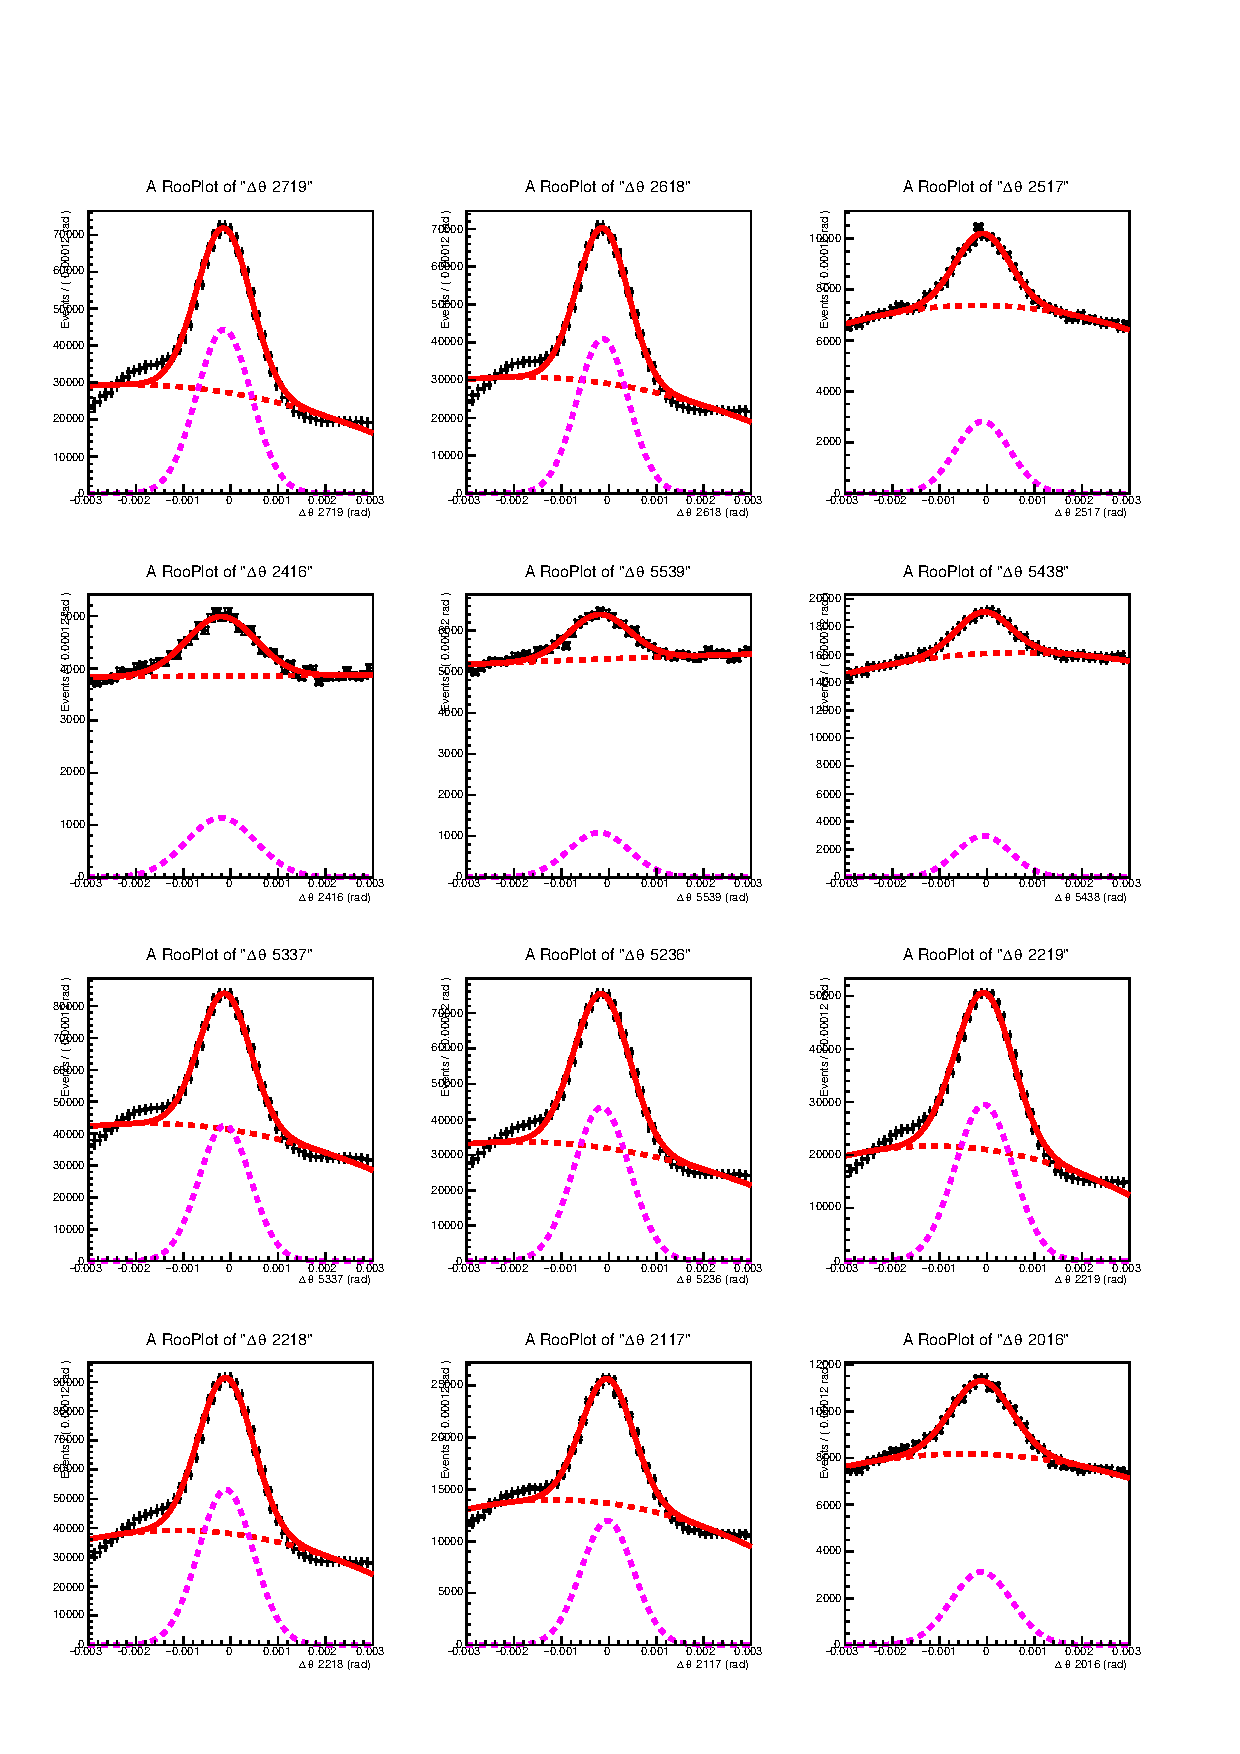
\includegraphics[width=1.\textwidth]{rich2_p1.pdf}
		\vspace*{-1.5cm}
	\end{center}
	\caption{\textit{Fit to the Cherenkov angle resolution distribution for RICH2 mirror-pairs.}}
	\label{fig:rich2p1}
\end{figure}
\clearpage
\begin{figure}[!h]
	\vspace*{-0.cm}
	\begin{center}
		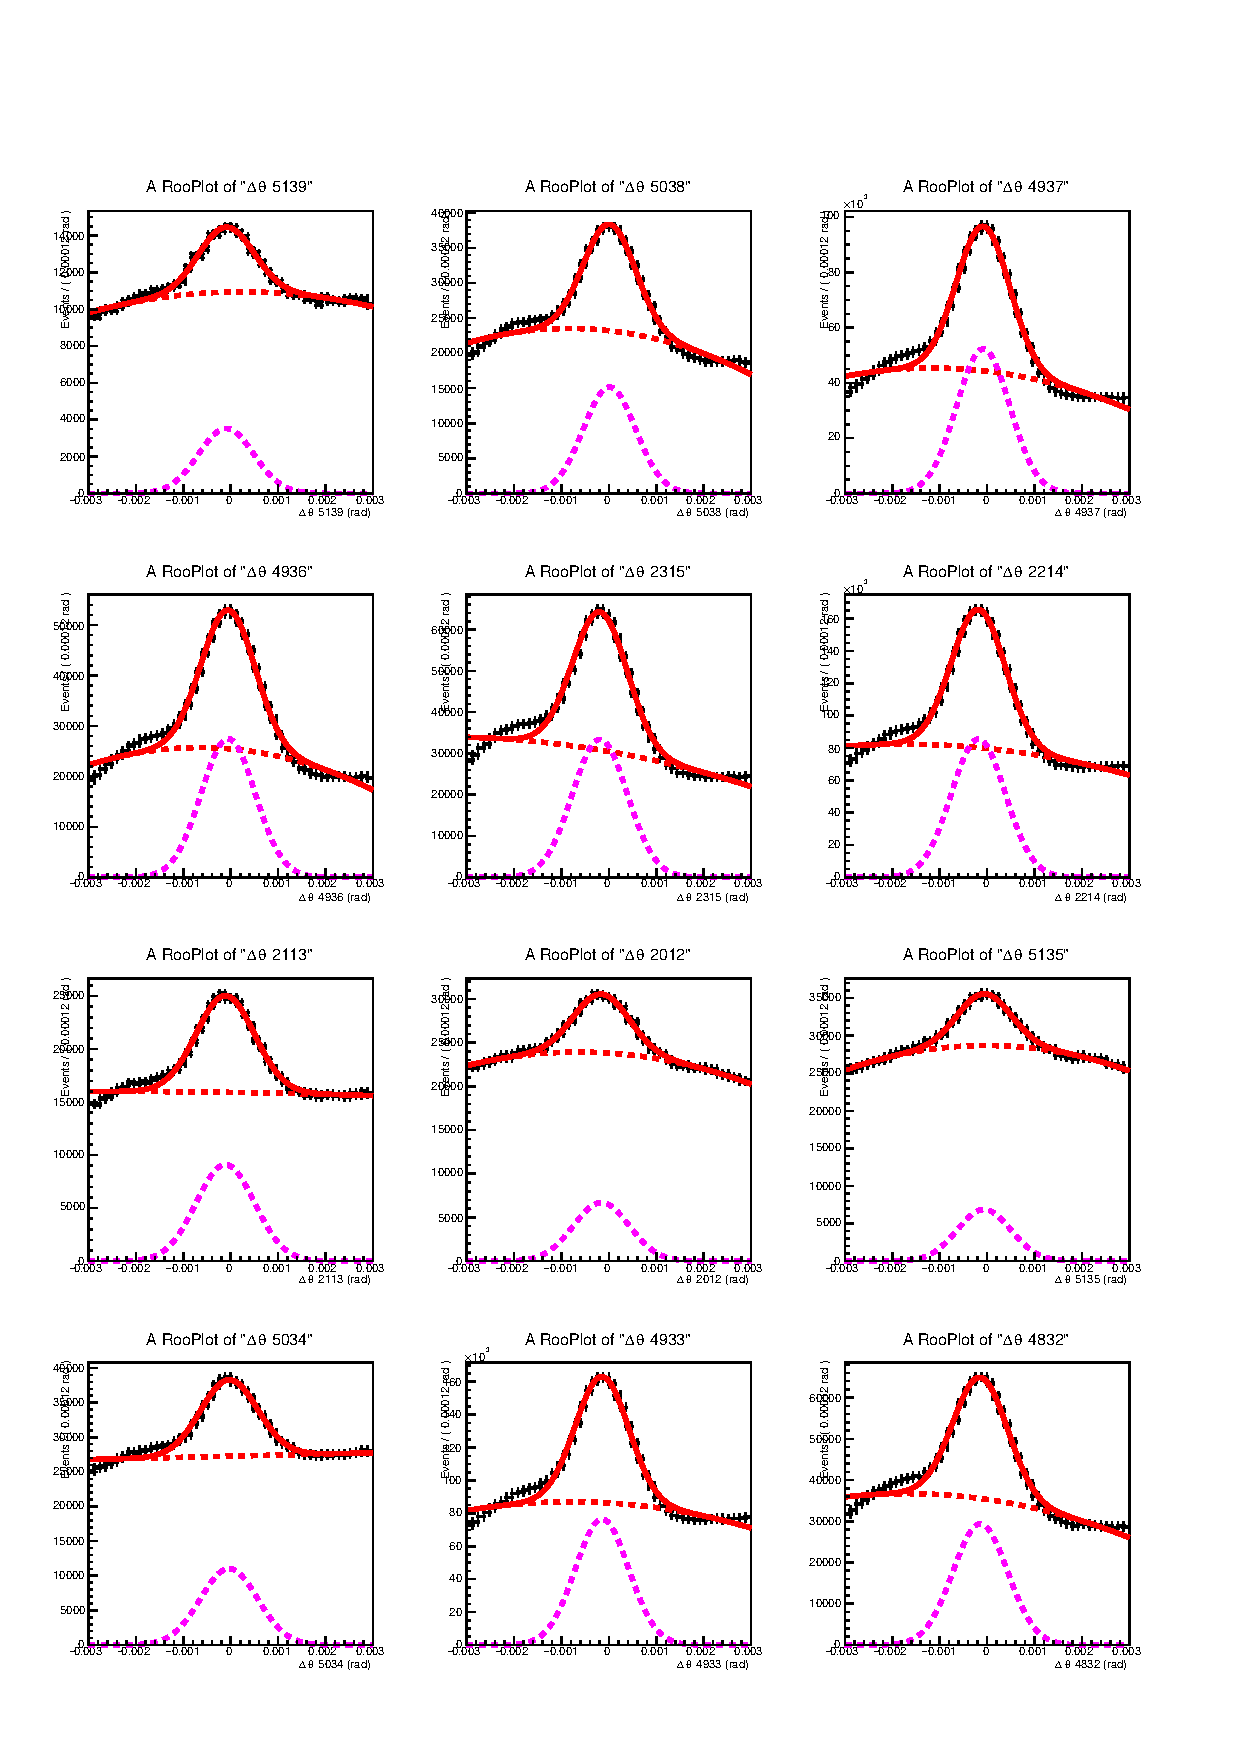
\includegraphics[width=1.\textwidth]{rich2_p2.pdf}
		\vspace*{-1.5cm}
	\end{center}
	\caption{\textit{Fit to the Cherenkov angle resolution distribution for RICH2 mirror-pairs.}}
	\label{fig:rich2p2}
\end{figure}
\clearpage
\begin{figure}[!h]
	\vspace*{-0.cm}
	\begin{center}
		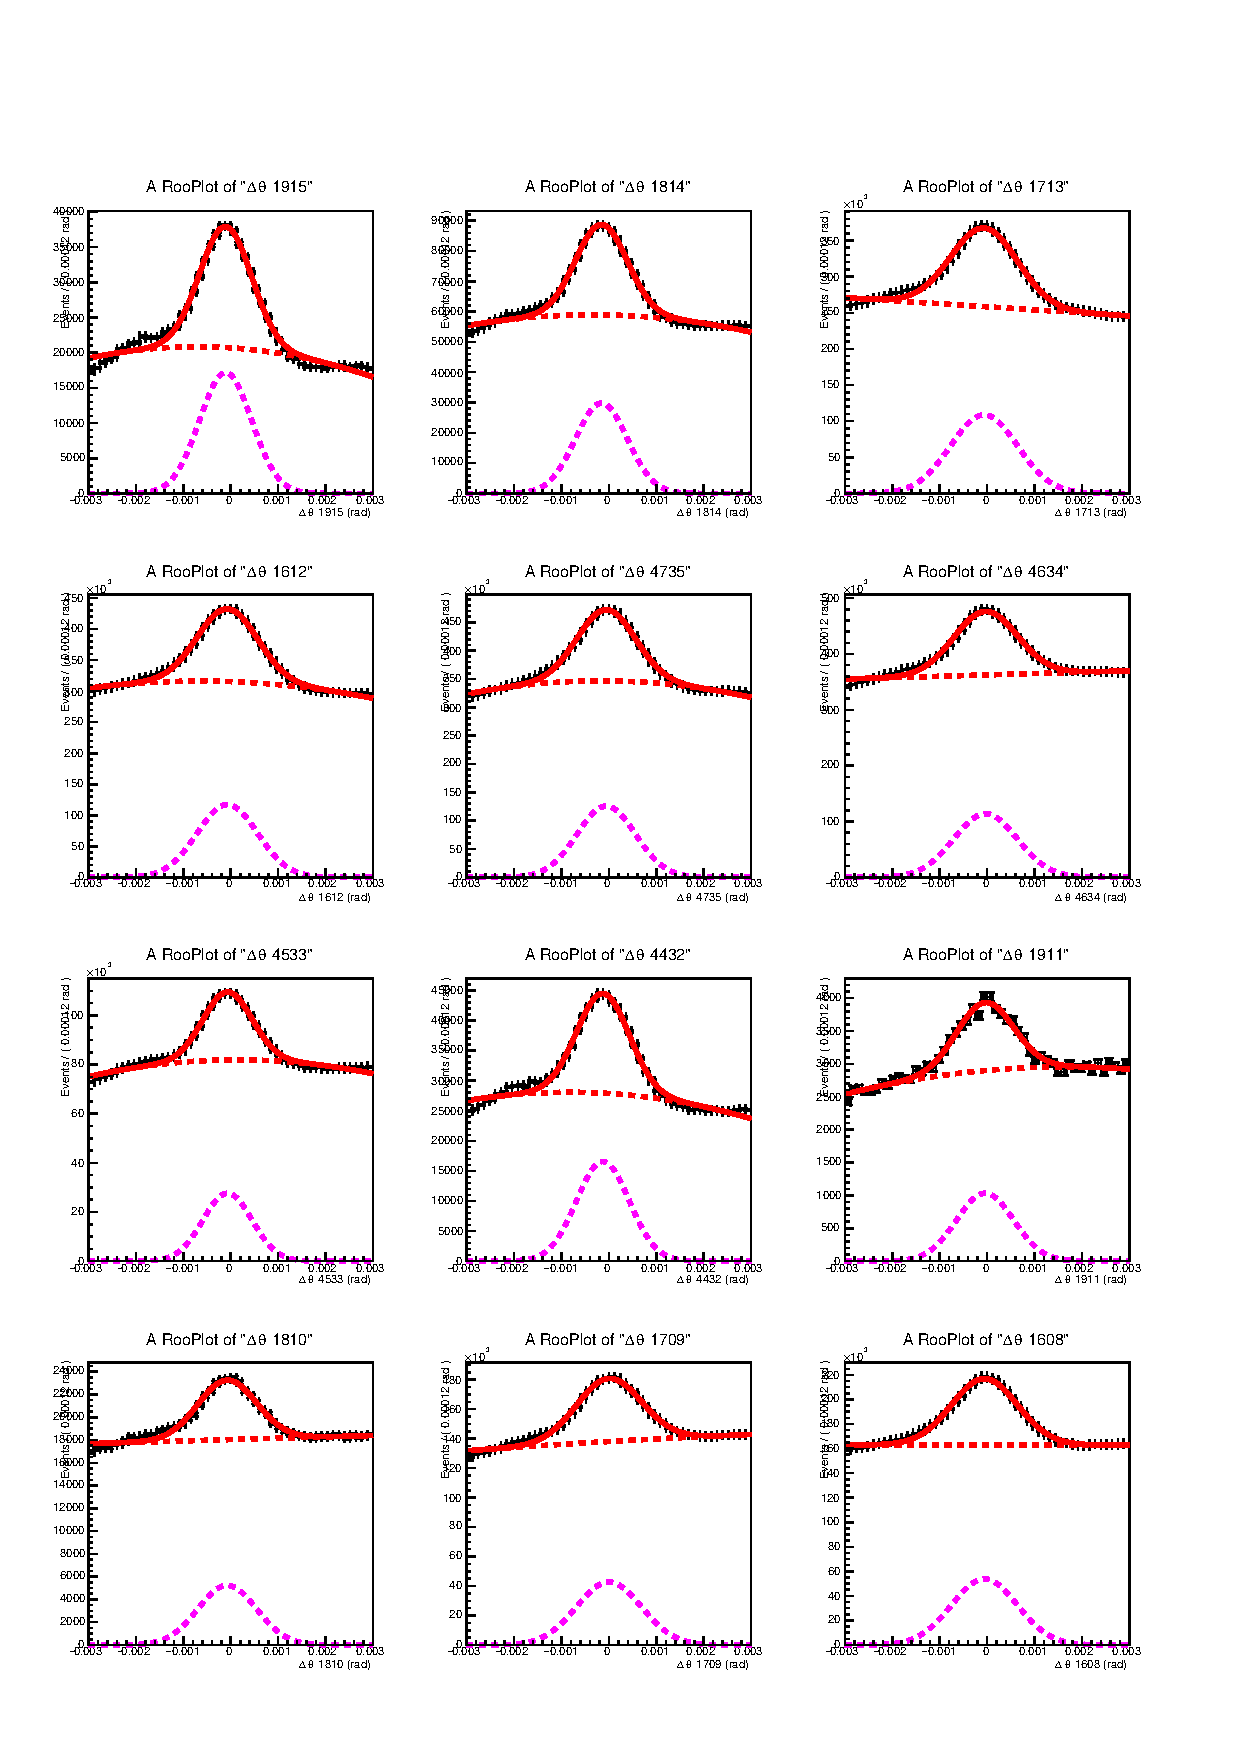
\includegraphics[width=1.\textwidth]{rich2_p3.pdf}
		\vspace*{-1.5cm}
	\end{center}
	\caption{\textit{Fit to the Cherenkov angle resolution distribution for RICH2 mirror-pairs.}}
	\label{fig:rich2p3}
\end{figure}
\clearpage
\begin{figure}[!h]
	\vspace*{-0.cm}
	\begin{center}
		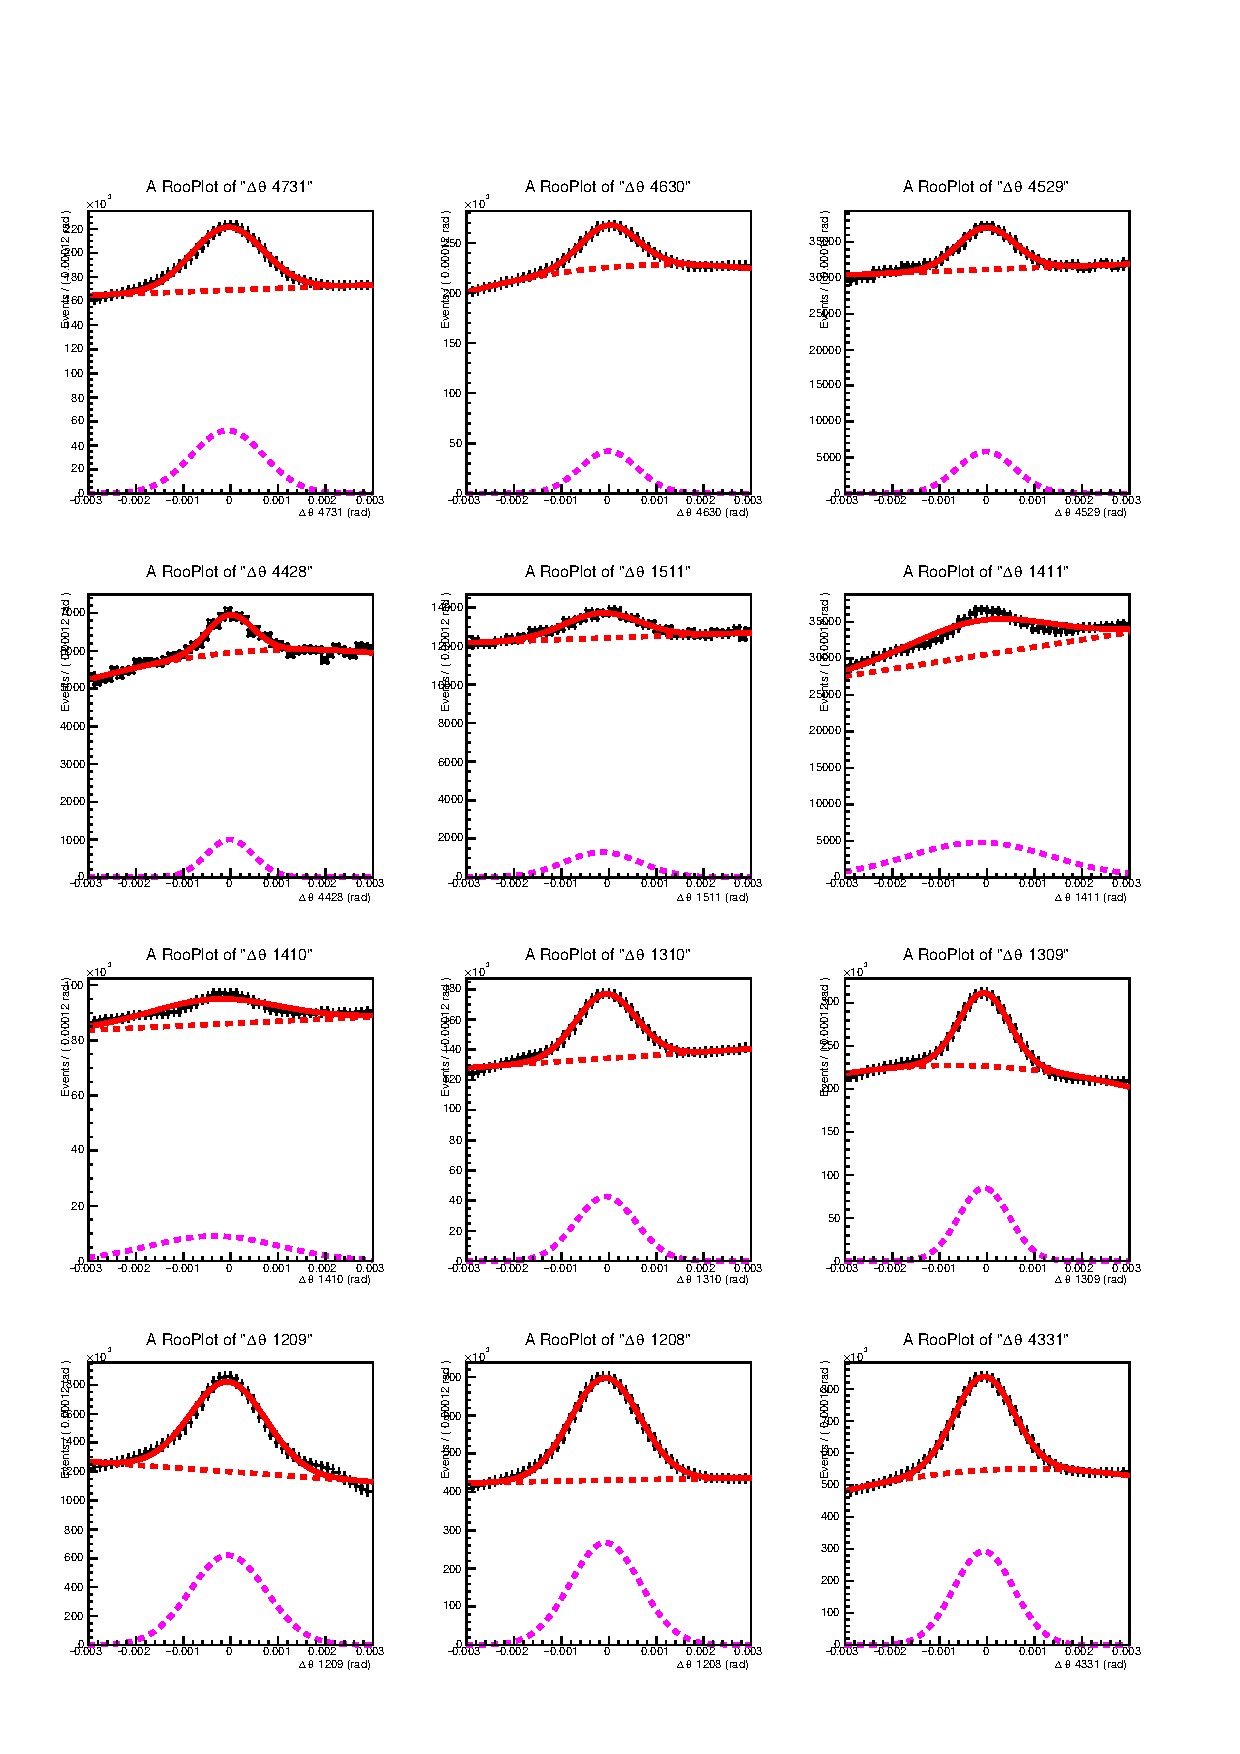
\includegraphics[width=1.\textwidth]{rich2_p4.pdf}
		\vspace*{-1.5cm}
	\end{center}
	\caption{\textit{Fit to the Cherenkov angle resolution distribution for RICH2 mirror-pairs.}}
	\label{fig:rich2p4}
\end{figure}
\clearpage
\begin{figure}[!h]
	\vspace*{-0.cm}
	\begin{center}
		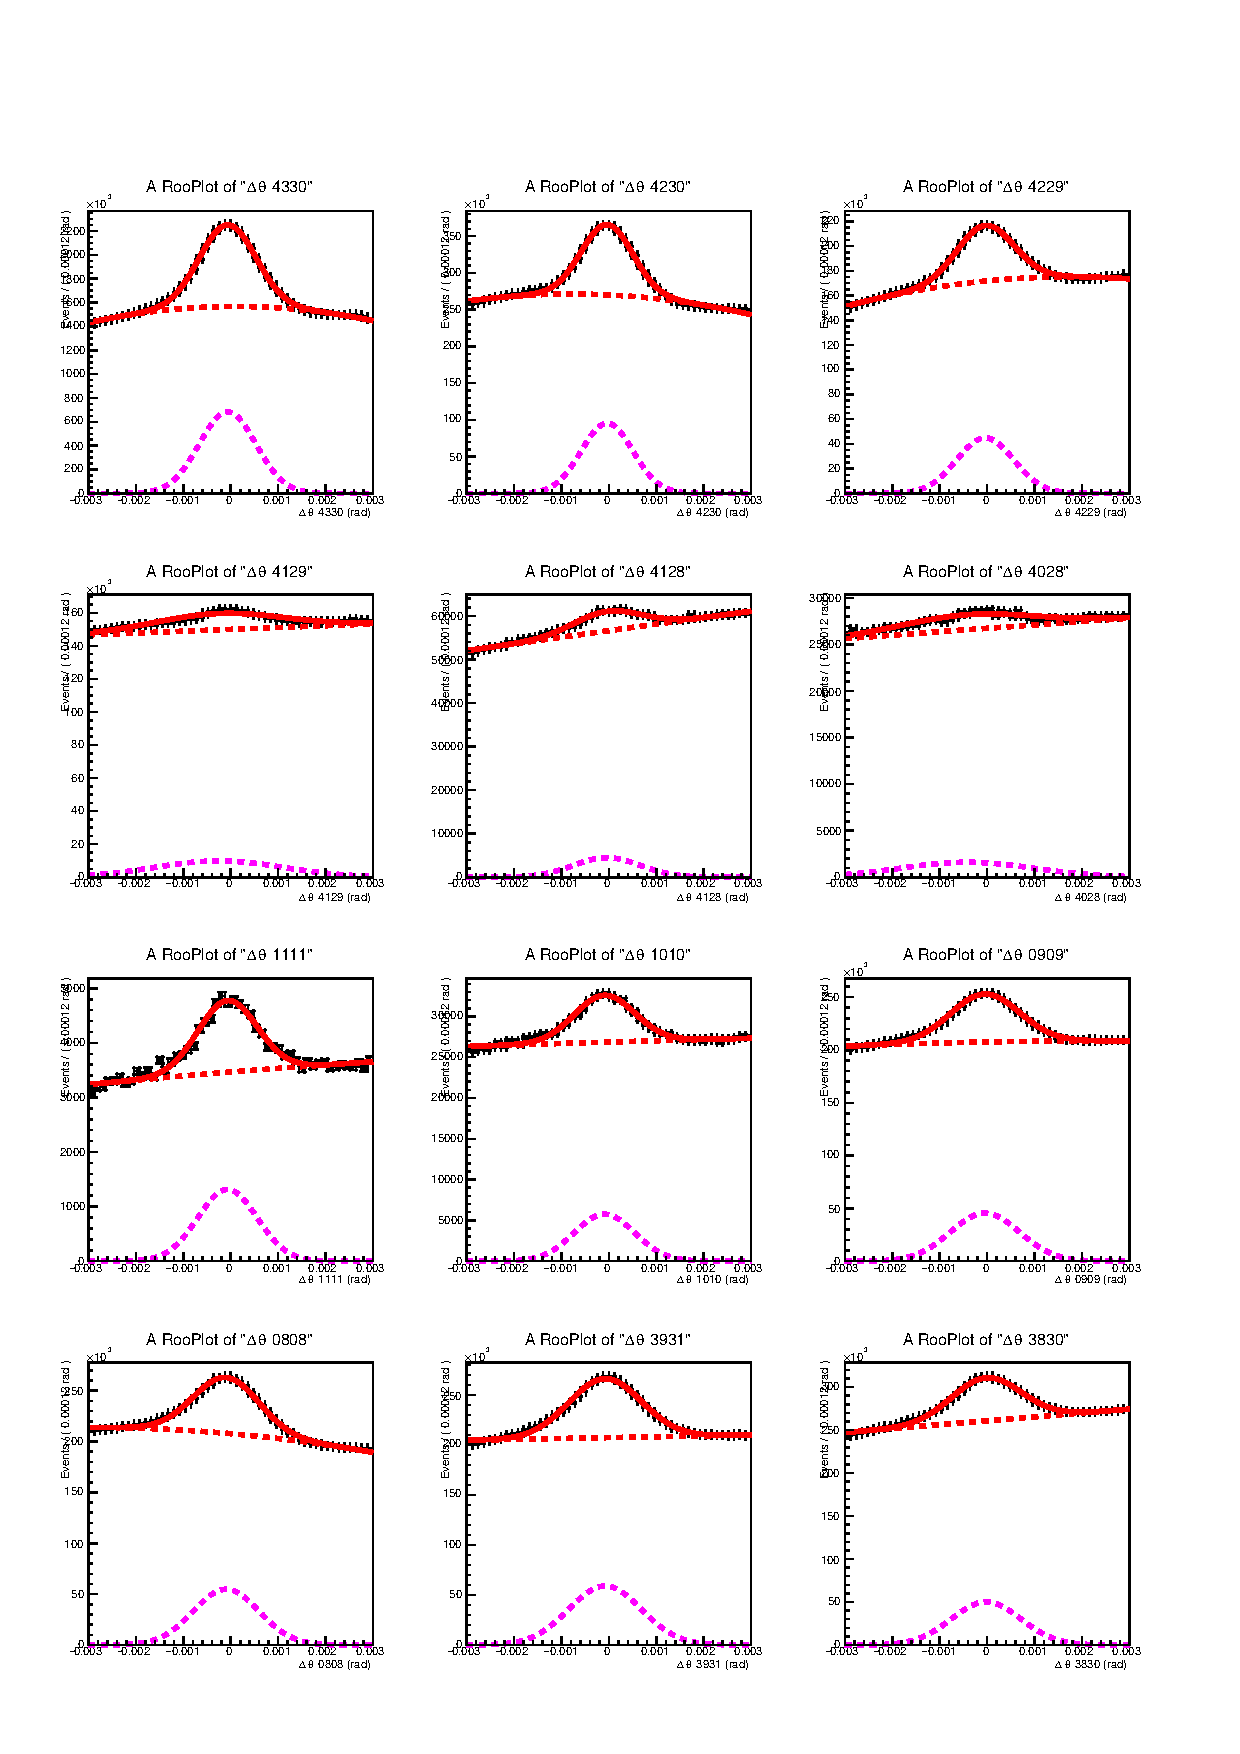
\includegraphics[width=1.\textwidth]{rich2_p5.pdf}
		\vspace*{-1.5cm}
	\end{center}
	\caption{\textit{Fit to the Cherenkov angle resolution distribution for RICH2 mirror-pairs.}}
	\label{fig:rich2p5}
\end{figure}
\clearpage
\begin{figure}[!h]
	\vspace*{-0.cm}
	\begin{center}
		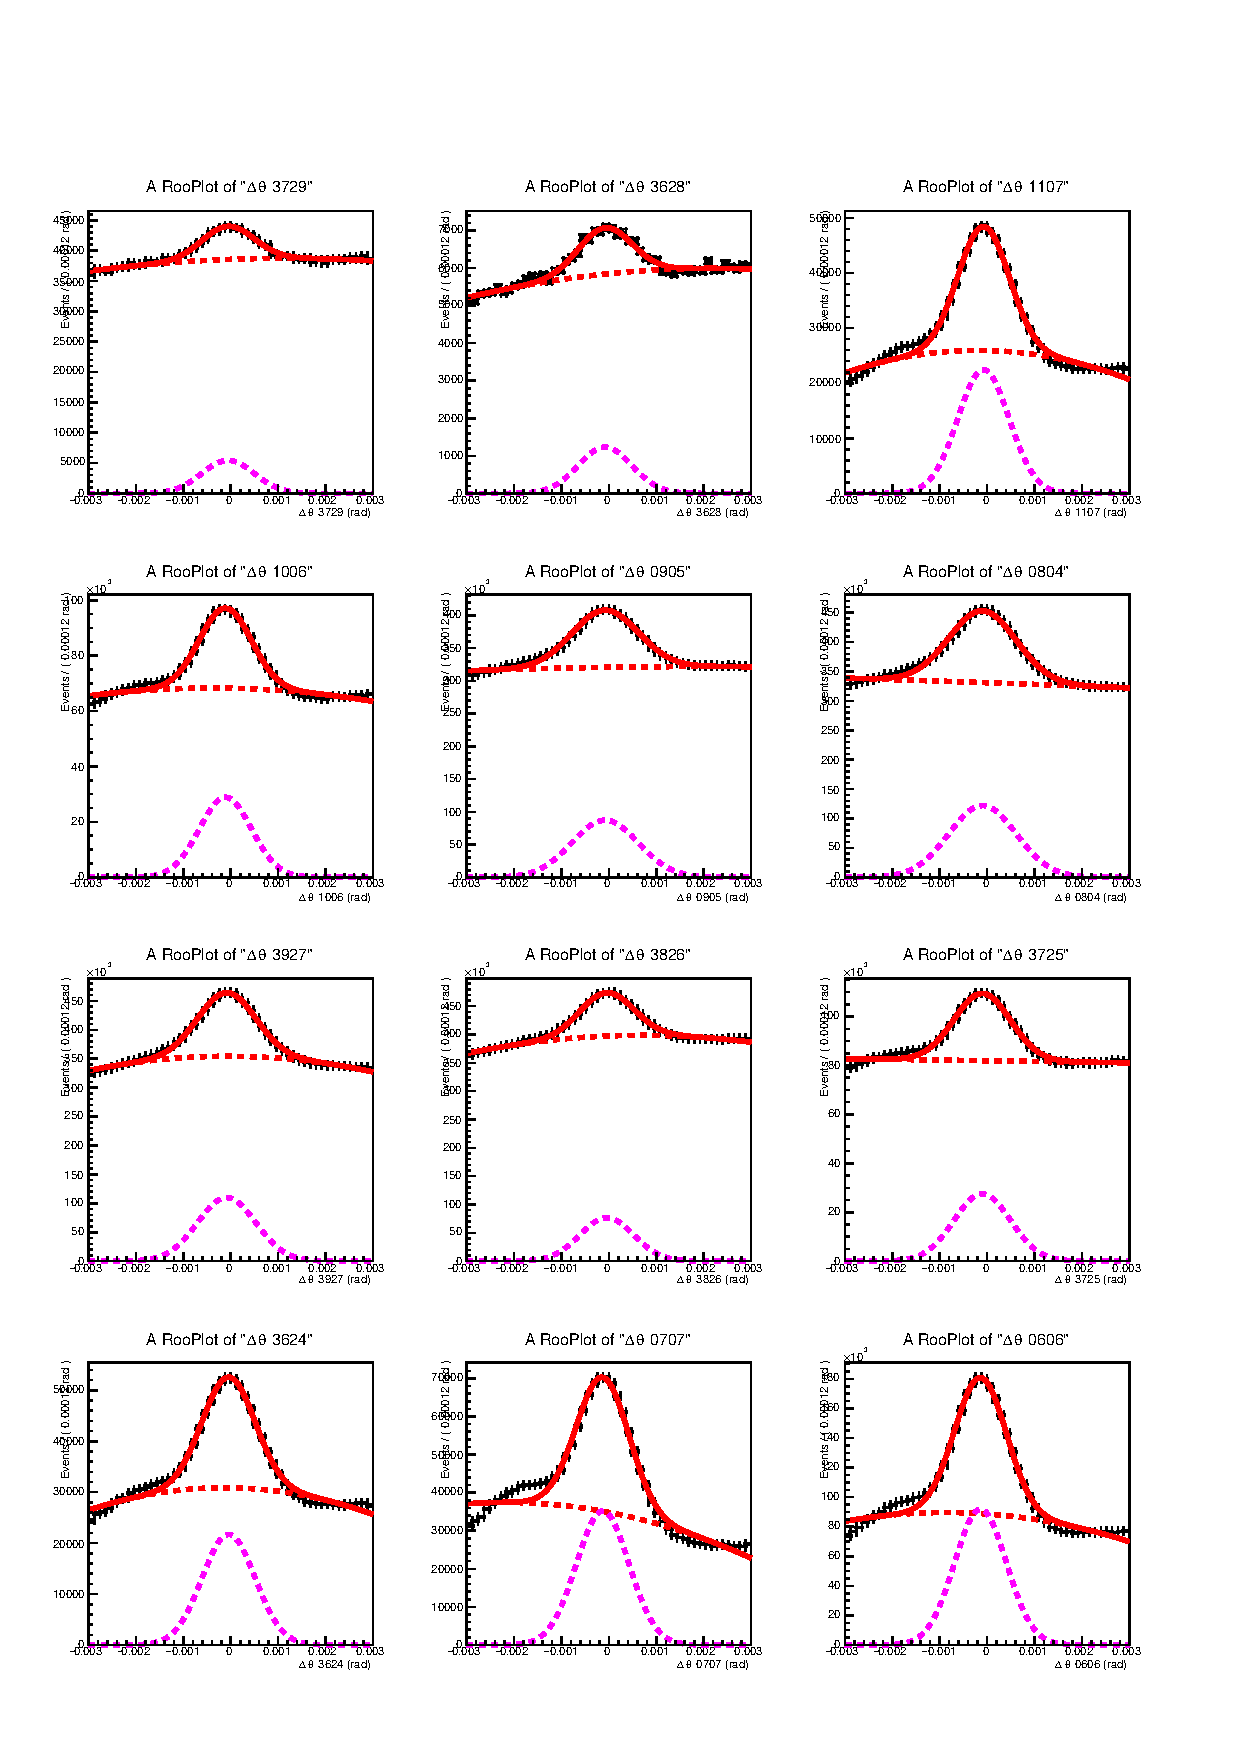
\includegraphics[width=1.\textwidth]{rich2_p6.pdf}
		\vspace*{-1.5cm}
	\end{center}
	\caption{\textit{Fit to the Cherenkov angle resolution distribution for RICH2 mirror-pairs.}}
	\label{fig:rich2p6}
\end{figure}
\clearpage
\begin{figure}[!h]
	\vspace*{-0.cm}
	\begin{center}
		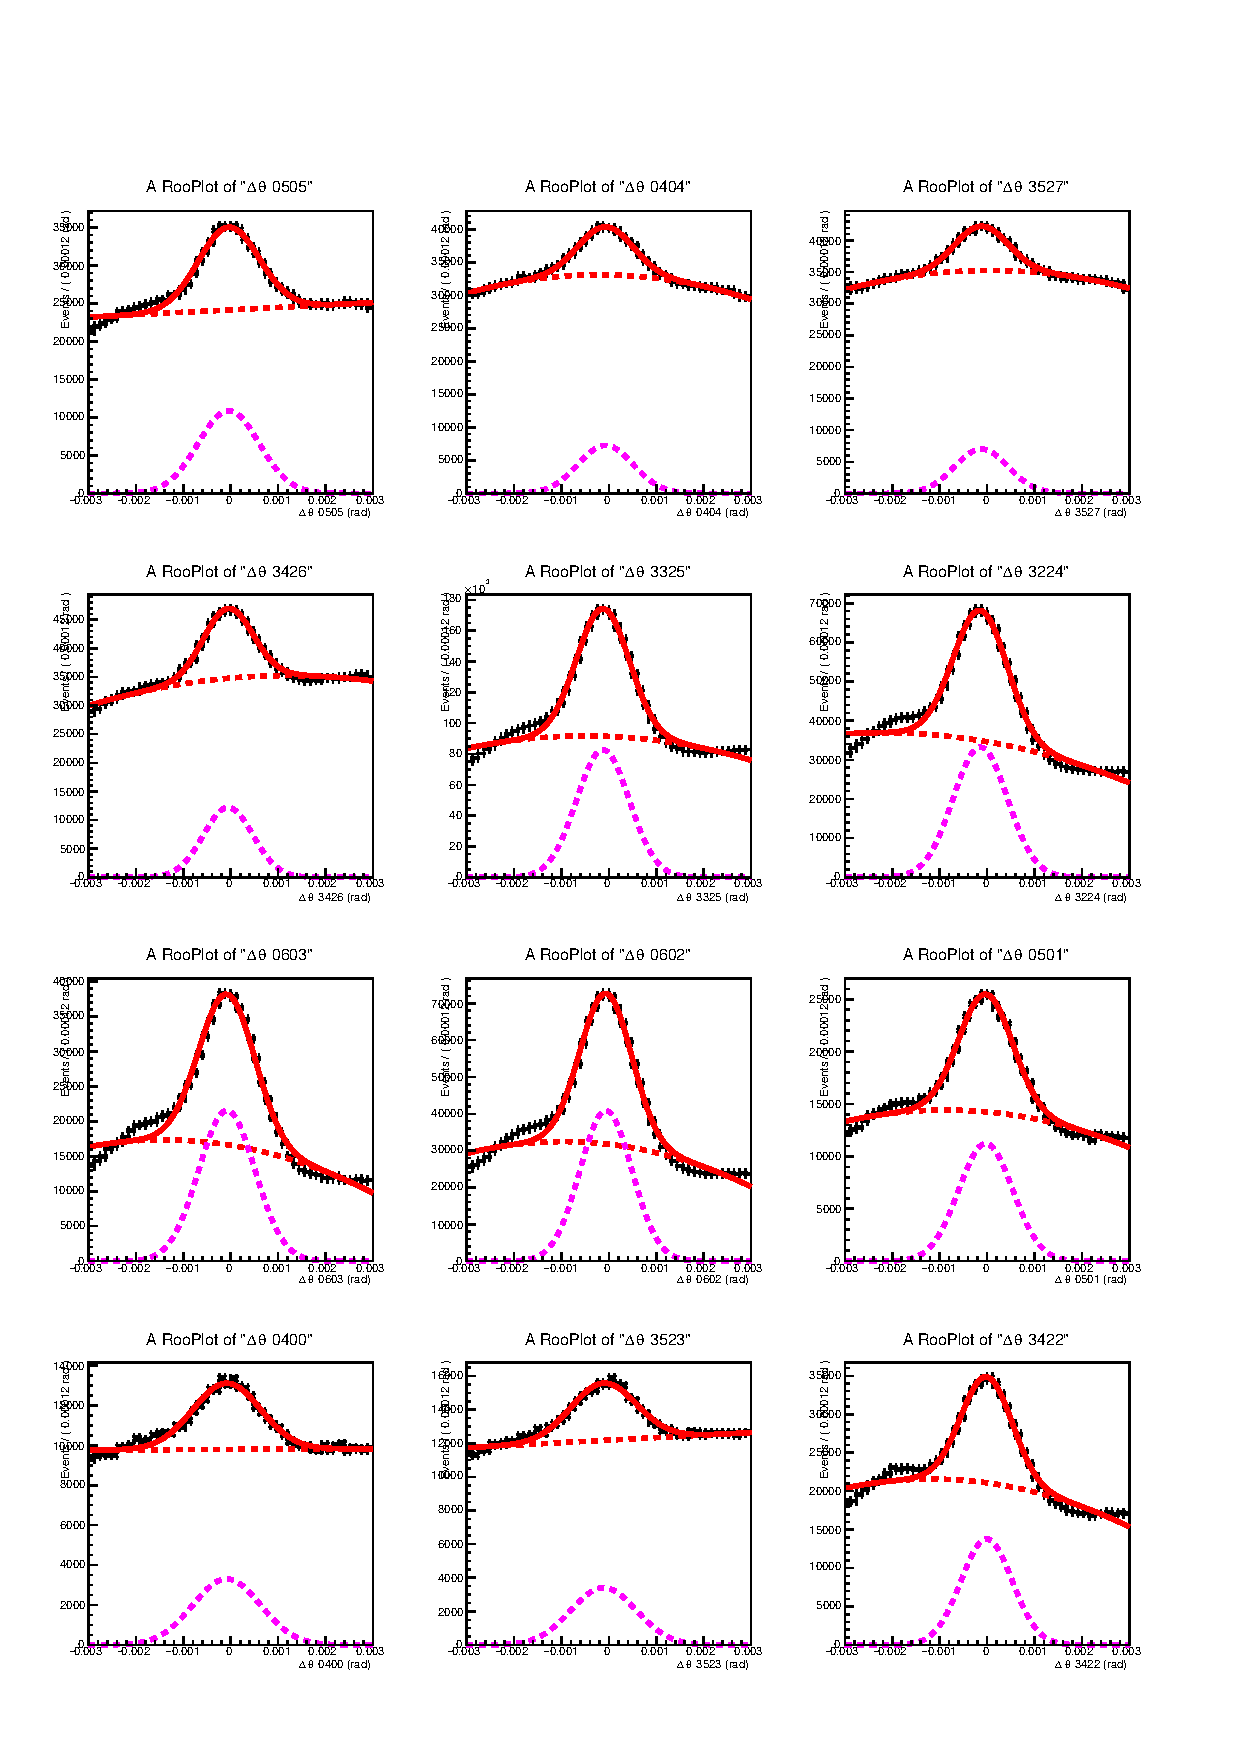
\includegraphics[width=1.\textwidth]{rich2_p7.pdf}
		\vspace*{-1.5cm}
	\end{center}
	\caption{\textit{Fit to the Cherenkov angle resolution distribution for RICH2 mirror-pairs.}}
	\label{fig:rich2p7}
\end{figure}
\clearpage
\begin{figure}[!h]
	\vspace*{-0.cm}
	\begin{center}
		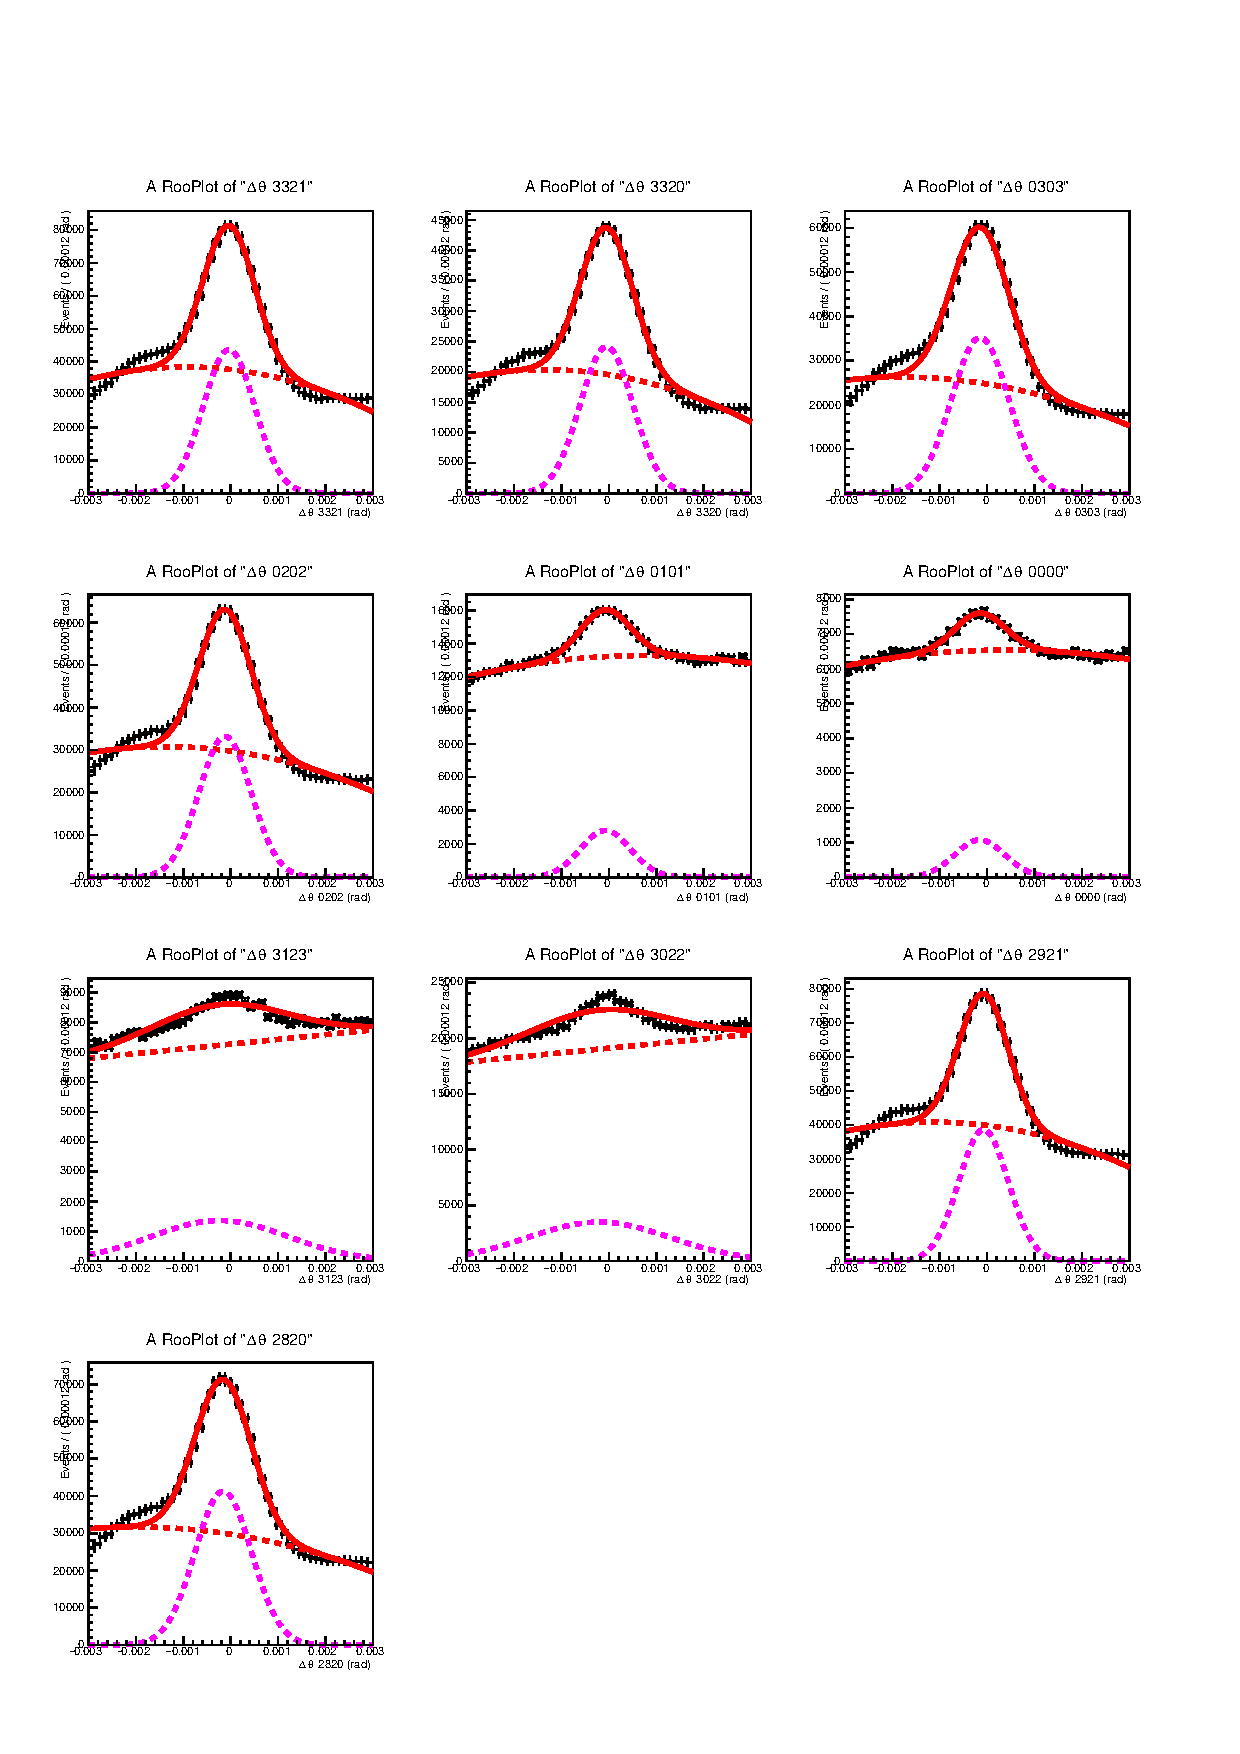
\includegraphics[width=1.\textwidth]{rich2_p8.pdf}
		\vspace*{-1.5cm}
	\end{center}
	\caption{\textit{Fit to the Cherenkov angle resolution distribution for RICH2 mirror-pairs.}}
	\label{fig:rich2p8}
\end{figure}